\documentclass[conf]{new-aiaa}
\usepackage{graphicx}
\let\Bbbk\relax
\usepackage{amsmath,amssymb}
\usepackage{booktabs}
\usepackage{xcolor}
\usepackage{subcaption}
\usepackage{multirow}
\newcommand{\todo}[1]{\textcolor{red}{\textit{[#1]}}}
\newcommand{\sm}{\mathrm{SM}}

\title{The Useful Emptiness: An Inboard Flap Gap as an Energy
       Concentrator for a Distributed-Propulsion eSTOL}

\author{Qiqi Wang\thanks{Co-founder, Flexcompute Inc.; Associate
        Professor, Department of Aeronautics and Astronautics,
        Massachusetts Institute of Technology; AIAA Associate
        Fellow.}}
\affil{Flexcompute Inc., Belmont, CA 94002, USA, and
       Massachusetts Institute of Technology, Cambridge, MA 02139, USA}
\author{Harry Smith\thanks{Director of Flight Sciences, Flexcompute Inc.;
        AIAA Member.}}
\affil{Flexcompute Inc., Belmont, CA 94002, USA}

% new-aiaa.cls's custom \maketitle drops the standard \@thanks flush,
% so \thanks{...} on \author{} produces only a footnote mark with no
% footnote text.  Patch it back in.
\makeatletter
\renewcommand{\maketitle}{%
  \begingroup
  \renewcommand\and{\\[\baselineskip]}%
  \centering\singlespacing
  {\LARGE\bfseries\@title\par}%
  \vskip2\baselineskip
  \@author\par
  \endgroup
  \vskip\baselineskip
  \if@journal\thispagestyle{empty}\fi
  \@thanks
  \global\let\@thanks\@empty
  \setcounter{footnote}{0}%
}
\makeatother

\begin{document}
\maketitle

\begin{abstract}
A 11.07-m-span, 2{,}600-lb ultra-STOL (uSTOL) aircraft with a
10-propeller distributed-electric propulsion array is studied
across cruise, takeoff, and landing using high-fidelity RANS CFD
(Flow360, actuator-disk thrust model).  Starting from the
naive low-htail / continuous-flap baseline (the X-57-class
layout, known to have stability shortcomings at high blowing),
we walk through a four-step configurational \emph{evolution}.
Step 1 raises the stabiliser to a high T-tail -- adequate at
today's published uSTOL approach envelopes but, when pushed
to the slower approach speeds and more aggressive flap
settings of this study, only weakly stable in takeoff and
mildly unstable in landing.  Subsequent steps then: (i) an inboard
flap gap that drives a centerline upwash column from the
streamwise vortices shed at the flap discontinuities; (ii) the
return of the horizontal tail into the prop slipstream column
for a $4$--$9\times$ local-q boost; and (iii) the shortening of
the tail boom -- enabled by the resulting stability headroom --
from $4\,c$ to $2\,c$ aft of the wing trailing edge.  The final
v3 configuration is stable in all phases (measured $\sm =
+15/+19/+21\%$ MAC cruise/takeoff/landing on the partial v3
sweep so far), trims the entire landing envelope
including high-thrust go-around within the htail stall margin,
allows aggressive landing rotation without tail strike, and
reduces both landing roll and go-around pitch transient.  The
full paper will add nonlinear phugoid dynamic simulations for
the three principal configurations and a CFD-resolved
ground-effect landing maneuver.
\end{abstract}

\section*{Nomenclature}
\noindent
\begin{tabular}{ll}
$\alpha$ & body angle of attack \\
$\theta_{ht}$ & horizontal-tail rotation (positive: TE down) \\
$T/L$ & delivered total thrust normalised by total lift; $L$ \\
       & \quad includes the thrust's vertical component, so $T/L = C_T / C_{L,\mathrm{total}}$ \\
       & \quad in the wind frame; pure CFD-derived dimensionless ratio \\
$C_L,C_D,C_{m_{\mathrm{CG}}}$ & lift, drag, and pitching-moment coefficients about CG \\
$\sm$ & static margin
       $\equiv -(\partial C_{m_{\mathrm{CG}}}/\partial\alpha) /
       (\partial C_L/\partial\alpha)$ \\
$\eta_t = q_{ht}/q_\infty$ & local-to-freestream dynamic-pressure ratio at the htail \\
$c_w$ & wing mean aerodynamic chord, $1.385\,$m \\
$b$ & wing span, $11.07\,$m
\end{tabular}

%====================================================================
\section{Introduction}
%====================================================================

Distributed-electric propulsion (DEP) over a high-lift wing
has opened a new class of \emph{ultra}-STOL (uSTOL) aircraft:
very short field performance at modest cruise wing loading,
enabled by blowing roughly half the aircraft weight directly
across the wing.  Electra's EL2 demonstrator and the
in-development EL9 hybrid are the most publicly visible
examples; both distribute eight to ten propellers along the
leading edge, deflecting Fowler-flap augmented section lift
coefficients well beyond $C_L = 4$.  The aerodynamic mechanism
by which leading-edge DEP improves take-off and high-lift
performance on a commuter-class platform has been quantified
in several recent studies \cite{Cusati2023DEPCommuter}.

The cost of DEP-augmented blown lift -- hidden in a clean
configuration drawing -- shows up at the empennage.  The same
propeller wake that creates wing $C_{L,\max}$ pours energetic,
deflected flow into the horizontal-tail region.  At high
thrust setting ($T/L \to 1$) the downwash blanket along the
centerline fills the airspace where the stabilizer would
operate, and elevator authority collapses precisely when it is
needed -- at low approach airspeeds, with flaps deployed, and
at the highest body angles of attack.

A simple low-mounted horizontal tail behind a continuous-flap
wing -- the layout adopted by the NASA X-57 ``Maxwell''
all-electric DEP testbed
\cite{Deere2017X57HighFidelity,Viken2017X57Airfoils,HwangNing2018X57MDO}
-- is known
to exhibit stability shortcomings at high thrust setting, and
is the natural starting point of any DEP-eSTOL configuration
study.  The textbook fix is to raise the stabilizer clear of
the wake (T-tail, high boom).  At the approach speeds and
flap settings representative of today's blown-lift uSTOL flight
envelopes this fix has proved adequate.  This paper, however,
targets a more aggressive uSTOL operating frontier -- slower
approach speeds, stronger blowing, and steeper landing flare
attitudes than current designs nominally accommodate -- and
shows that within that extended envelope \emph{the T-tail fix
is necessary but insufficient}: even with a $40\%$-span,
full-chord stabilizer perched at $z=+1.9\,c_w$ and extending
from $x=+3.5\,c_w$ to $+4.5\,c_w$ aft of the CG
(i.e.\ $4\,c_w$ aft of the wing leading edge), the
configuration remains unstable in landing (and only weakly
stable in takeoff).  We then walk through
a four-step \emph{evolution} that arrives at a much better
configuration for this extended envelope: starting from the
X-57-style cont-low baseline (Step~0), raise the htail (Step~1,
the current wisdom), introduce an inboard flap gap
(Step~2), drop the horizontal tail back into the slipstream
column to harvest the slipstream dynamic pressure
(Step~3, ironically returning to the Step~0 vertical position),
and -- once the stability headroom is large enough -- shorten
the tail boom (Step~4).

We perform an unsteady RANS sweep with Flow360
\cite{Fitzgibbon2025HLPW5,Fitzgibbon2022HLPW4,Fitzgibbon2023DPW7,Casses2022BlownPropPropulsion,Jia2023RotorFundamentals,Jia2021TiltrotorDES}
on a 10-prop, $165\,$ft$^2$, $2{,}600\,$lb reference uSTOL at ISA
$3{,}658\,$m.  The three phases run at $(V_\infty,\gamma)$ of
$(45.7\,$m/s, $0)$ cruise, $(18.0\,$m/s, $+30^\circ)$ takeoff,
and $(12.9\,$m/s, $-30^\circ)$ landing, with sensitivity
sweeps centred on baseline
$(\alpha,\theta_{ht},T_{\mathrm{mult}})$ of $(+7,0,1)$,
$(+8,-5,16)$, $(+8,-6,12)$ respectively (BO $T/L$ of $0.05$,
$0.52$, $0.39$).  Three high-lift section airfoils
(Fig.~\ref{fig:airfoils}) form a Fowler-deployed assembly; the
inboard $40\%$ span is optionally a ``flap gap.''  The four
configurations form a $2\times 2$ design matrix in
$(\text{flap continuity}, z_{ht})$ (Fig.~\ref{fig:configs}).
Per combination and phase we run an
$\alpha$/$\theta_{ht}$/$T/L$ sensitivity sweep, fit local
linear sensitivities with stall-point masks, and solve the
$3\times 3$ trim system for the equilibrium flight condition.

\begin{figure}[htb!]
  \centering
  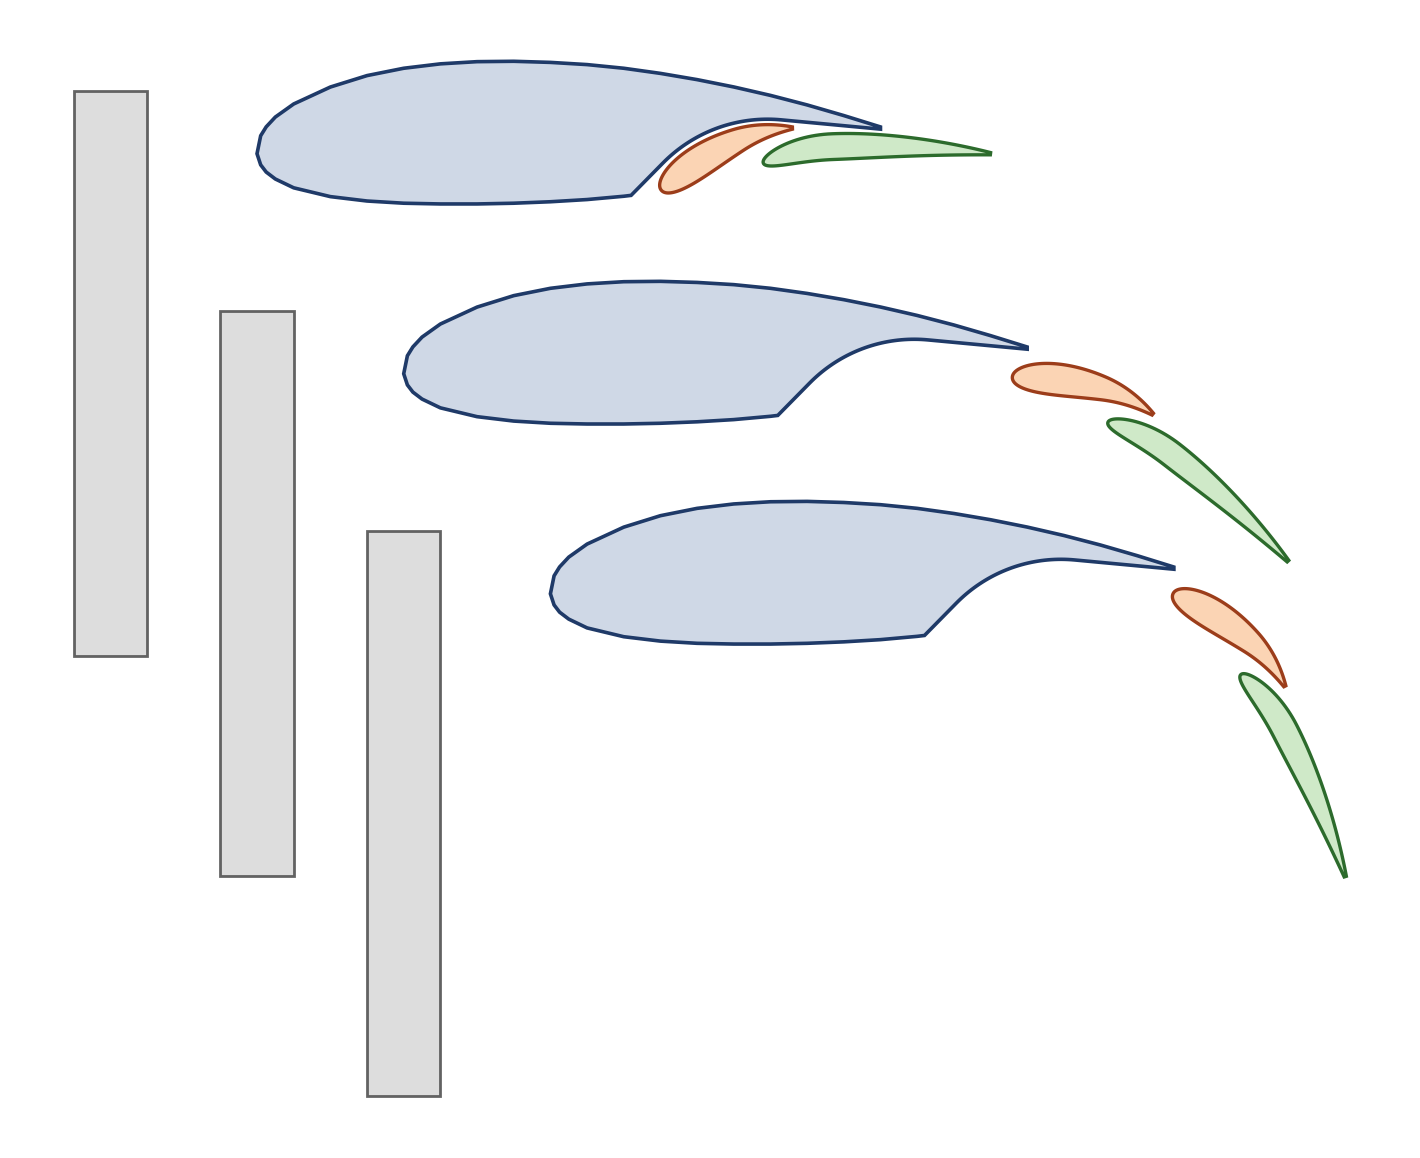
\includegraphics[width=0.55\linewidth]{figures/airfoil_phases_stacked.png}
  \caption{Three-element high-lift system in three Fowler
           kinematic states (top to bottom: stowed, takeoff,
           landing).  Coved LS(1)-0417 main element, NACA 9621
           vane, and NACA 6311 aft flap; each successive
           configuration is shifted downward by $0.3\,c$.  The
           gap-flap variants omit the vane + aft-flap assembly
           across the central $40\%$ of the wing span.}
  \label{fig:airfoils}
\end{figure}

\begin{figure}[htb!]
  \centering
  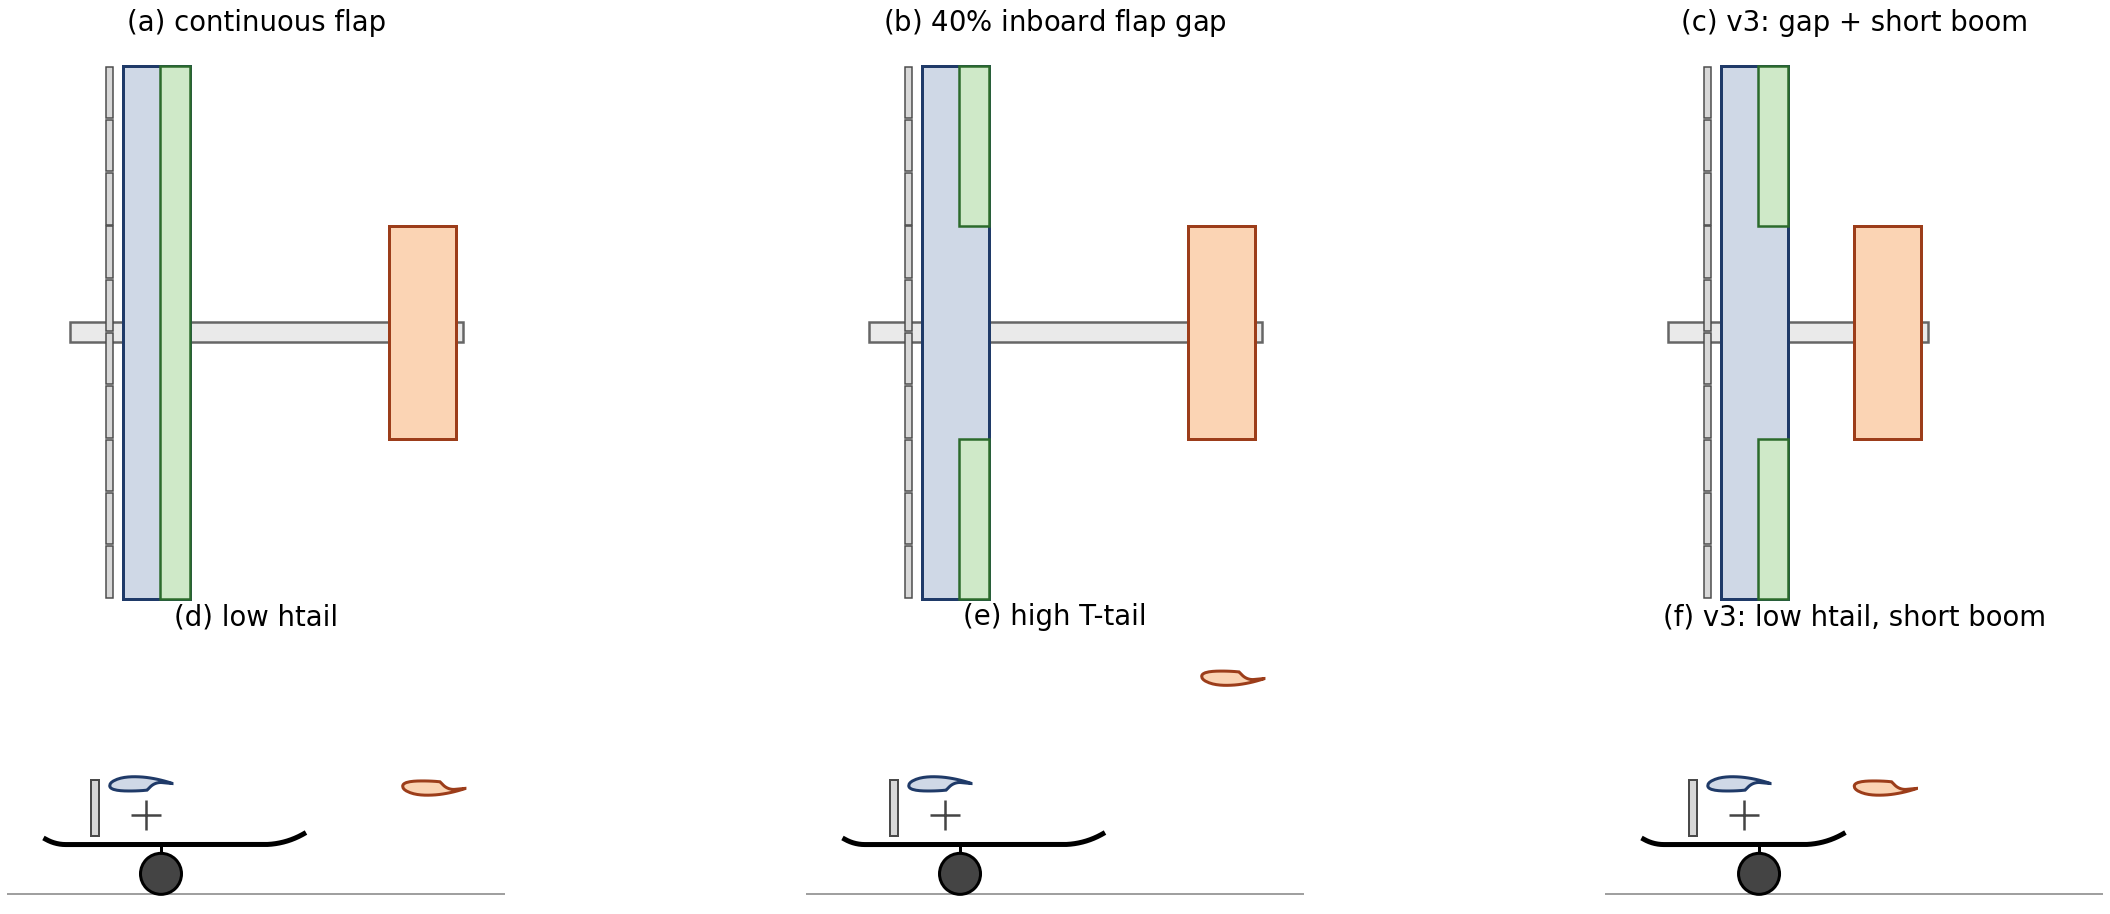
\includegraphics[width=\linewidth]{figures/config_montage.png}
  \caption{Configuration evolution at the cruise (flap-stowed)
           reference geometry.  Top row, top views: (a)
           continuous flap; (b) $40\%$ inboard flap gap; (c)
           gap + shortened tail boom (v3, principal proposal).
           The top views are independent of the horizontal-tail
           vertical position.  Bottom row, side views: (d) low
           horizontal tail; (e) high T-tail; (f) v3 low htail
           with the shortened boom.  Wing and horizontal-tail
           sections shown at actual chord scale (clean
           LS(1)-0417 for the wing; inverted LS(1)-0417 for
           the htail).  Actuator disks are drawn as rectangles
           (axial-thickness $\times$ projected-diameter) so
           they appear physically correct in both projections.
           CG is marked ``+''; main landing gear shown as a
           filled circle.  The same gear is drawn in all three
           side views to highlight the rotational advantage of
           the short-boom v3: at high landing-flare attitudes
           the aircraft pitches up around the main-gear contact
           point, and the shorter-arm htail in (f) clears the
           ground at flare attitudes where the long-boom
           configurations (d, e) would strike.}
  \label{fig:configs}
\end{figure}

%====================================================================
\section{Configurational Evolution}
\label{sec:evolution}
%====================================================================

\paragraph{\textbf{Note on grid uniformity.}}
\label{sec:caveats}
The CFD sweeps that feed Table~\ref{tab:sm} and the downwash
slices (Figs.~\ref{fig:downwash-cont-low}--\ref{fig:downwash-v3})
were carried out at each configuration's own equilibrium trim
point rather than on a single shared $(T/L, \theta_{ht})$
grid: the landing slices sit at $T/L\approx 0.60$ for cont-low,
$0.39$ for cont-high and gap-high, and at the respective BO
values for gap-low and v3.  Because slipstream downwash scales
with $T/L$, cross-configuration magnitudes and $\sm$ deltas
inherit a thrust-dependent bias of unknown sign; the
\emph{directions} of the effects we report (gap-induced
upwash, slipstream $q$-boost, short-boom moment-arm penalty)
are robust to this bias, but quantitative cross-configuration
deltas should be read as indicative.  The full paper will rerun
every configuration on a common $(T/L, \theta_{ht})$ grid and
report calibrated deltas.  The downwash plots also use a
body-fixed slice (perpendicular to body $x$ at
$x_b{=}+4.4\,$m) with Flow360's freestream pinned along world
$+x$ and the airframe rotated by $\theta$ via the
\texttt{ac\_pitch} rotation cylinder, so the plotted
$\epsilon=\arctan(-w_\mathrm{world}/u_\mathrm{world})$ is
measured against the freestream direction and the htail dotted
line sits at constant $z_\mathrm{body}$ across all $\alpha$
panels.

\subsection{Step 0 -- The Naive Low-Tail Baseline (cont-low)}

The simplest DEP-eSTOL configuration places a conventional
low-mounted horizontal tail behind a continuous-flap wing.
This is the layout of the NASA X-57 ``Maxwell'' all-electric
DEP testbed
\cite{Deere2017X57HighFidelity,Viken2017X57Airfoils,HwangNing2018X57MDO},
the most publicly visible example of which is known to have
experienced flight-readiness challenges that contributed to the
program's 2023 closure.
For our 10-prop, full-span distributed array this layout
is fine in unflapped cruise -- a clean, lightly-loaded wing
and a tail outside the (small) prop wake gives a textbook
$\sm = +46.7\%$ MAC.  The failure modes the X-57 community
anticipated emerge in the flapped phases:
Figure~\ref{fig:cont-low-sens} shows the sensitivity sweeps
across the three phases.  In takeoff and landing the
horizontal tail sits inside the wing+flap downwash and is
hit by the wakes of the inboard propellers; both contribute
to a destabilising downwash gradient that erodes the tail's
restoring moment.  The static-margin column of
Table~\ref{tab:sm} reads $\sm = +2.9\%$ in takeoff (barely
stable) and $\sm = -19.5\%$ in landing (strongly unstable);
cont-low sets the benchmark against which the subsequent steps
are measured.

\begin{figure}[htb!]
  \centering
  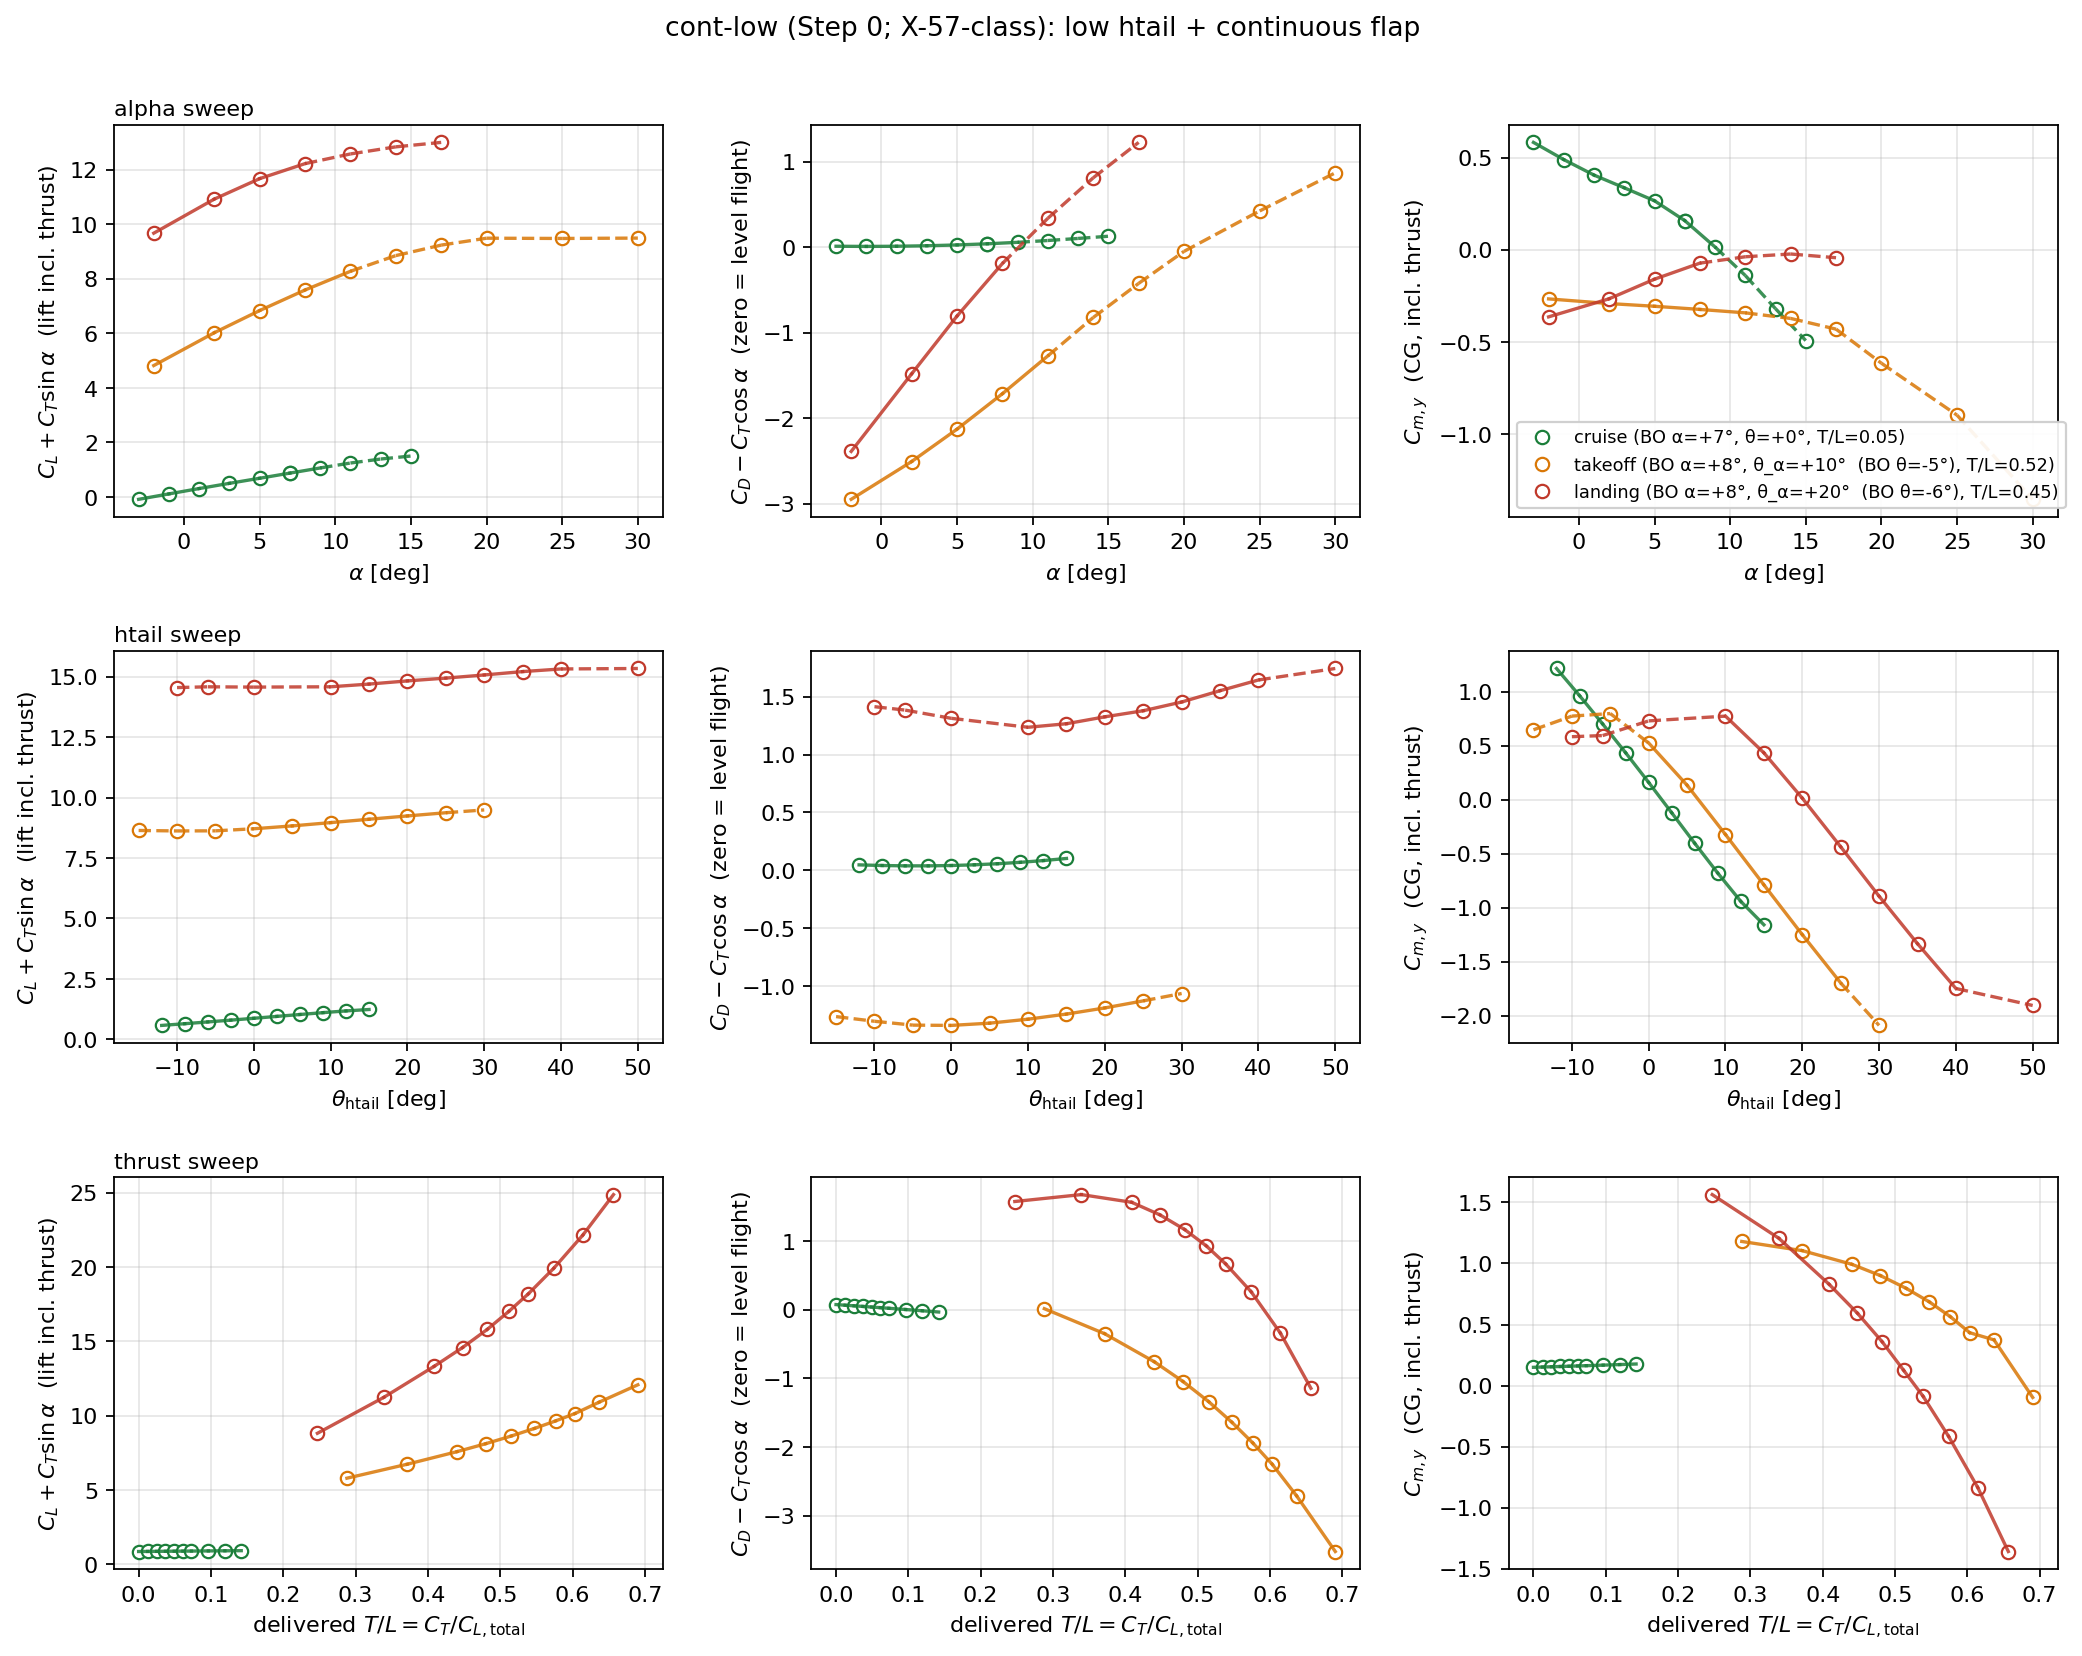
\includegraphics[width=\linewidth]{figures/cont_low_combined_sens.png}
  \caption{Sensitivity sweeps for the cont-low Step~0
           baseline (the X-57-class layout) with all three
           flight phases overlaid on a common set of axes:
           \textcolor[HTML]{1b7e3a}{cruise} (green),
           \textcolor[HTML]{d97706}{takeoff} (orange),
           \textcolor[HTML]{c0392b}{landing} (red).  Lift and
           drag columns include the streamwise thrust
           contribution:
           $C_{L,\mathrm{total}} = C_L + C_T \sin\alpha$ and
           $C_{D,\mathrm{total}} = C_D - C_T \cos\alpha$, so
           that $C_{D,\mathrm{total}} = 0$ marks level flight
           (climb when negative, descent when positive).  The
           $C_{m_{\mathrm{CG}}}$-vs-$\alpha$ slope in the third
           column is positive in both takeoff and landing,
           indicating instability; cruise on the clean wing is
           comfortably stable.  Cont-low sets the benchmark
           against which the subsequent steps are measured.}
  \label{fig:cont-low-sens}
\end{figure}

The downwash field at the htail station makes the
static-margin numbers physical.
Figure~\ref{fig:downwash-cont-low} shows the wind-frame
downwash angle
$\epsilon = \tan^{-1}(-w_\mathrm{world}/u_\mathrm{world})$ on a
body-fixed yz-slice $0.45\,$m upstream of the htail leading
edge at landing trim, for two angles of attack
($\alpha=+5^\circ$ and $+17^\circ$).  Reading $\epsilon$
along the htail dotted line ($z_\mathrm{body}=+0.554\,$m): at
$\alpha=+5^\circ$ the htail sits in $\epsilon\approx
+45^\circ$ downwash, and at $\alpha=+17^\circ$ it sits in
$\epsilon\approx +55^\circ$.  A $12^\circ$ increase in body
$\alpha$ thus produces a $\sim 10^\circ$ increase in
downwash at the htail, so the effective $\alpha$ seen by the
htail rises by only $\sim 2^\circ$ -- the htail is almost
completely shielded from the body's pitch motion, and the
$\sm = -19.5\%$ landing entry of Table~\ref{tab:sm}
follows directly.  An upward gust on the airframe is
intercepted by the downwash blanket before it can produce
the htail restoring moment a low-DEP-loading aircraft would
rely on.

\begin{figure}[htb!]
  \centering
  \includegraphics[width=\linewidth]{figures/downwash_cont_low.png}
  \caption{Wind-frame downwash $\epsilon$ at the cont-low
           htail station ($x_b = $ htail LE $-0.45$ m,
           landing trim, $T/L \approx 0.60$), at
           $\alpha=+5^\circ$ (left) and $\alpha=+17^\circ$
           (right).  Labeled contour lines are degrees of
           $\epsilon$; the dotted black line marks the htail
           span at its body-z station.  The htail sits inside a
           deep downwash column ($\epsilon \gtrsim +20^\circ$)
           -- the geometric mechanism behind the cont-low
           landing instability.}
  \label{fig:downwash-cont-low}
\end{figure}

\subsection{Step 1 -- The Current Wisdom: T-Tail with Continuous Flap (cont-high)}

The traditional remedy is to lift the stabiliser clear of the
wake: cont-high replaces the low htail with a T-tail at
$z=+1.9\,c_w$, recovering elevator effectiveness through a
reduced downwash gradient.  Figure~\ref{fig:cont-high-sens}
shows the sensitivity sweeps across the three phases.

\begin{figure}[htb!]
  \centering
  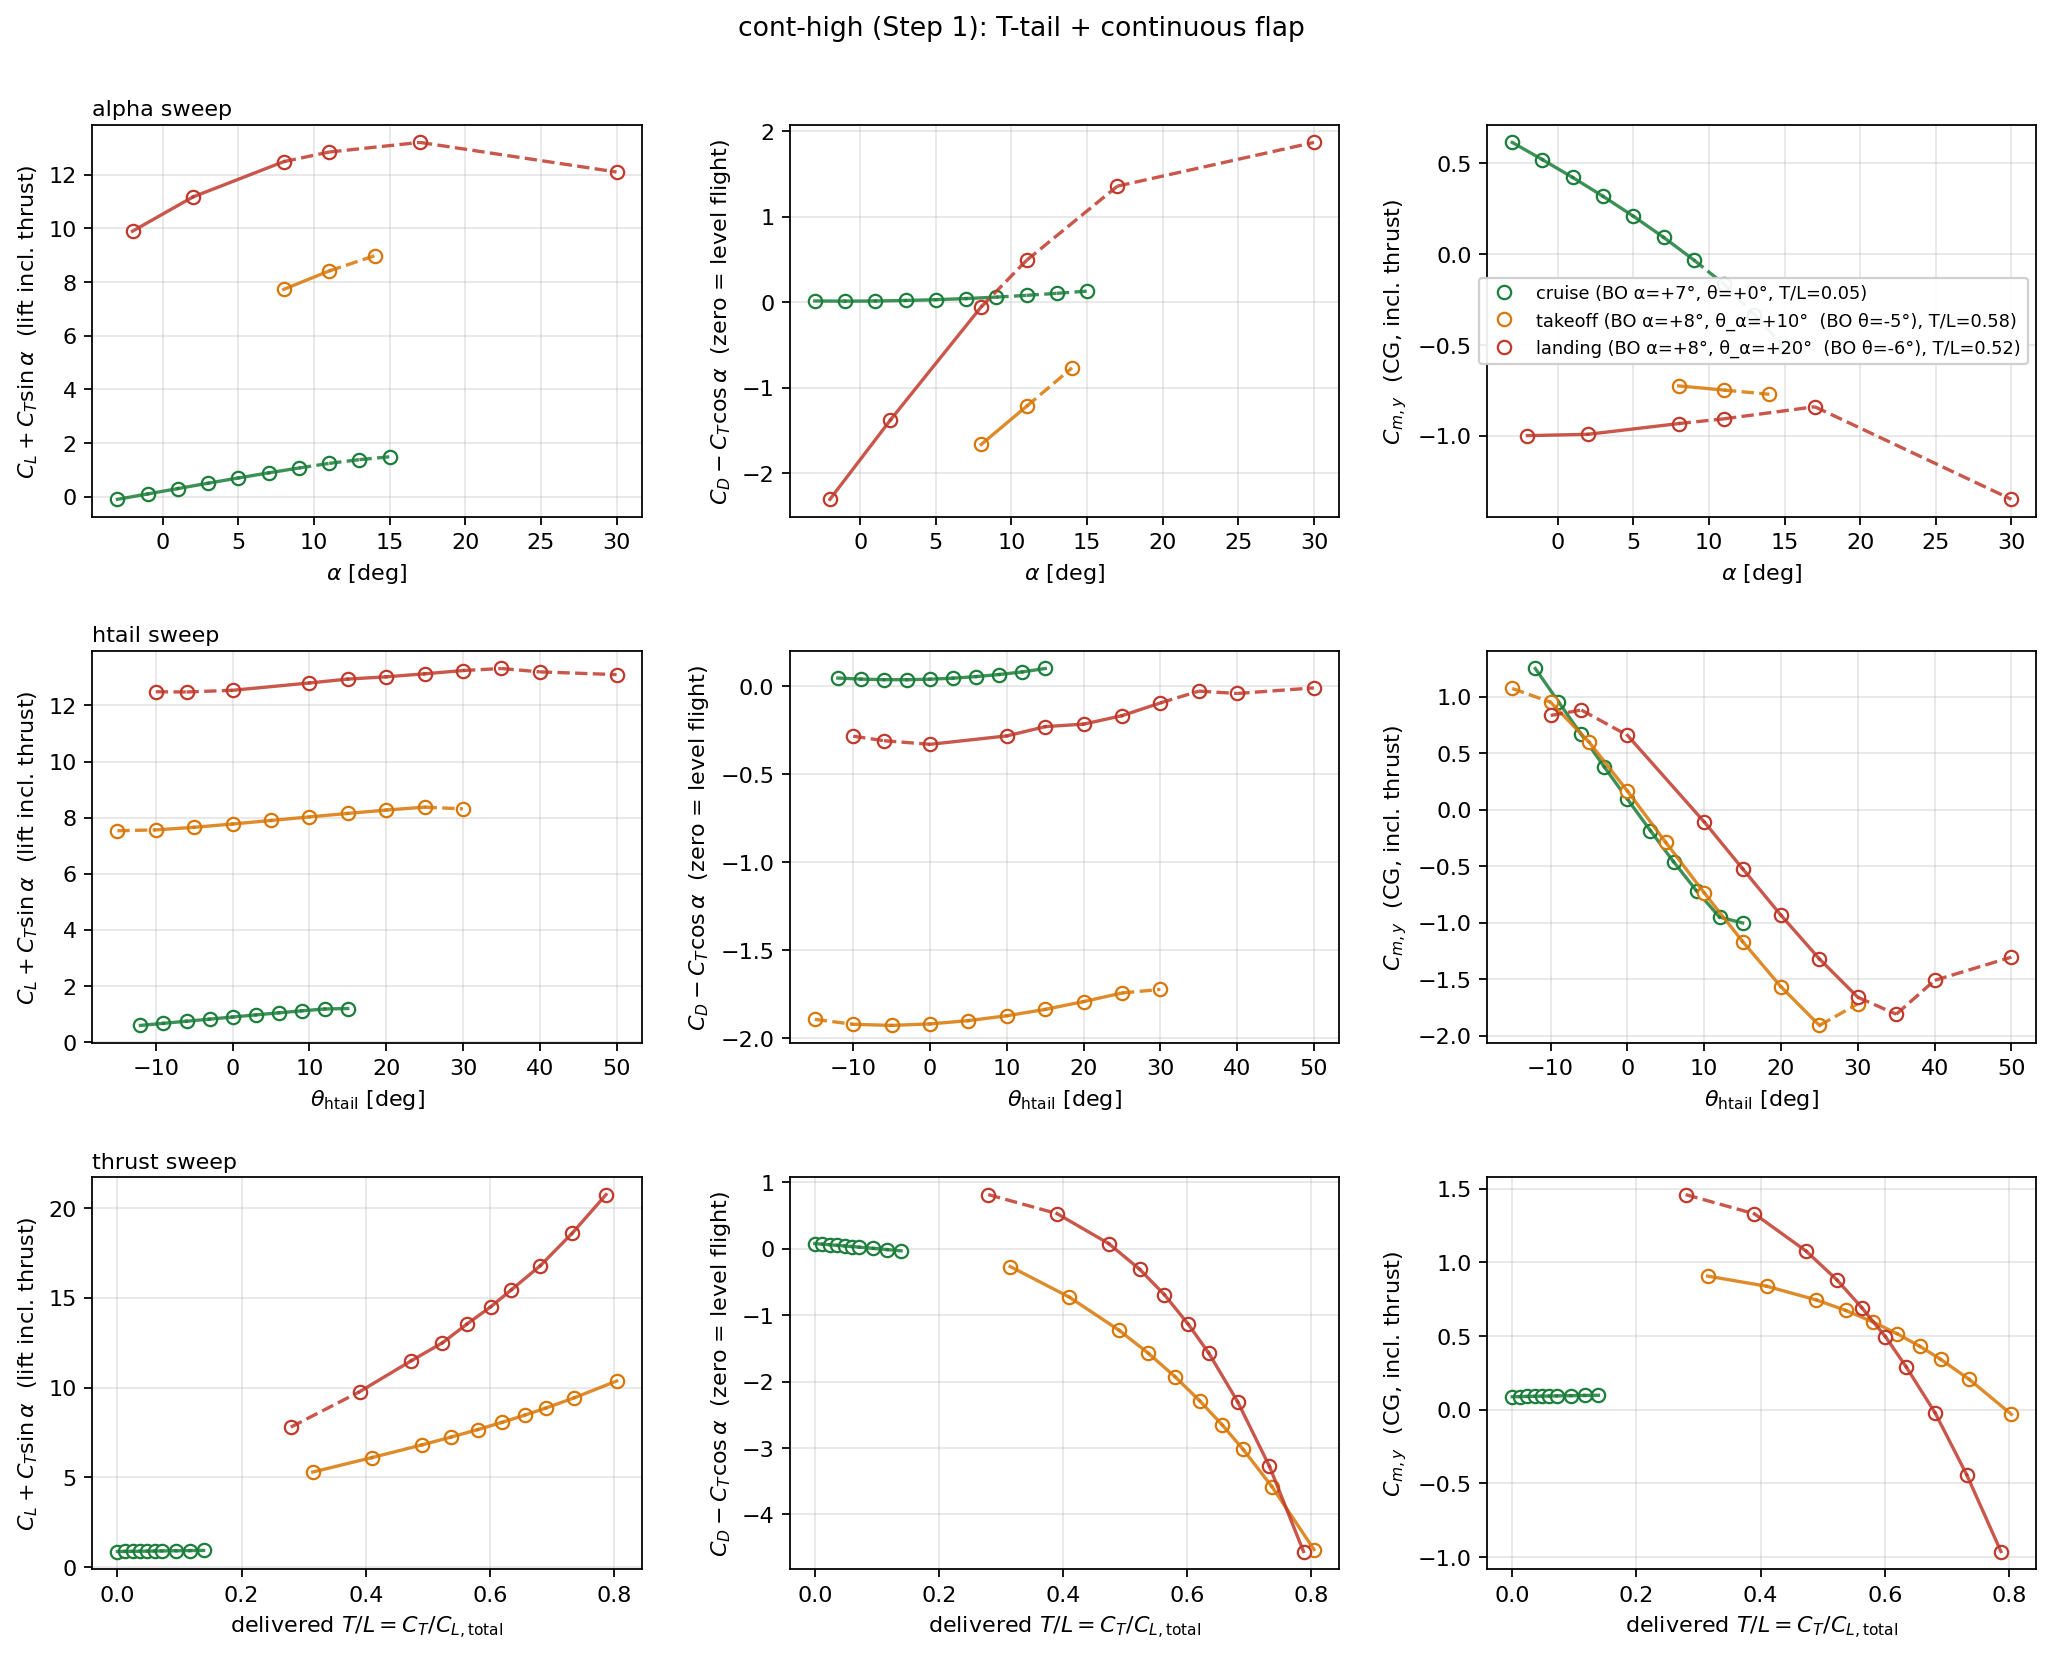
\includegraphics[width=\linewidth]{figures/cont_high_combined_sens.png}
  \caption{Sensitivity sweeps for the cont-high T-tail
           baseline (Step~1), three flight phases on common
           axes: \textcolor[HTML]{1b7e3a}{cruise} (green),
           \textcolor[HTML]{d97706}{takeoff} (orange),
           \textcolor[HTML]{c0392b}{landing} (red).  Rows are
           the three sensitivity sweeps ($\alpha$,
           $\theta_{ht}$, $T/L$); the first two columns are
           $C_{L,\mathrm{total}} = C_L + C_T\sin\alpha$ and
           $C_{D,\mathrm{total}} = C_D - C_T\cos\alpha$, so
           $C_{D,\mathrm{total}}=0$ corresponds to level flight.
           Solid line segments lie inside the linear-fit
           range; dashed segments lie outside.  See
           Table~\ref{tab:sm} for the static-margin entries.}
  \label{fig:cont-high-sens}
\end{figure}

Three uSTOL-relevant observations follow:

\begin{enumerate}
  \item The T-tail buys back stability in cruise but \emph{not}
        in landing -- exactly the phase that stresses
        empennage authority most.
  \item Elevator authority (coefficient slope) is similar in
        cruise and landing for cont-high
        ($|\partial C_{m_{\mathrm{CG}}}/\partial\theta_{ht}|
        \approx 0.087$/deg cruise, $0.078$/deg landing -- only
        $\sim 10\%$ lower at landing).  In \emph{dimensional}
        terms, however, the moment authority $q\cdot S \cdot c \cdot
        |dC_m/d\theta_{ht}|$ scales with $q$, and the landing
        $q$ is $(V_\mathrm{land}/V_\mathrm{cruise})^2 = (12.86/
        45.72)^2 \approx 8\%$ of cruise.  Despite the stabiliser
        being $40\%$ of the wingspan and full main-wing chord
        (large by any conventional metric), the marginal trim
        deflections sit close to the empirical htail stall
        boundary ($+12^\circ$ takeoff, $+20^\circ$ landing).
  \item In the negative-$\sm$ landing regime, the htail
        operates at high lift to trim the wing+flap moment.
        If the htail stalls in this state -- e.g.\ during a
        flare gust upset -- $|\partial C_{m_{\mathrm{CG}}}/\partial\theta_{ht}|$
        collapses to zero, the wing+flap nose-down moment is
        unopposed, and the aircraft enters a nose-diver
        attitude with no static-recovery path.  This is a
        catastrophic failure mode at landing altitude.
\end{enumerate}

The textbook fix is necessary, but at the extended-envelope
landing condition this paper targets it does not deliver a
credible safety margin.  At today's published Electra-class
approach speeds the same configuration would be acceptable;
the analysis above is best understood as describing what
happens when one tries to push a conventional empennage beyond
its current operating frontier.

The downwash field shows the partial nature of the fix.
Figure~\ref{fig:downwash-cont-high} shows wind-frame
$\epsilon$ on the same upstream-of-htail yz-slice, with the
htail now at $z_\mathrm{body}=+2.63\,$m.  Reading the dotted
line, the htail sits in $\epsilon\approx +30^\circ$ at
$\alpha=+5^\circ$ and $\epsilon\approx +37^\circ$ at
$\alpha=+17^\circ$.  A $12^\circ$ body-$\alpha$ increase now
produces only a $\sim 7^\circ$ downwash increase at the htail,
so the htail's effective $\alpha$ rises by $\sim 4$--$5^\circ$
-- a meaningful (but mild) improvement over cont-low's
$\sim 2^\circ$.  The T-tail clears the densest core of the
wing-flap downwash but only blunts, rather than reverses, the
landing-destabilising gradient: the residual
$d\epsilon/d\alpha > 0$ at the htail is the geometric
explanation for the still-unstable landing entry in
Table~\ref{tab:sm}.

\begin{figure}[htb!]
  \centering
  \includegraphics[width=\linewidth]{figures/downwash_cont_high.png}
  \caption{Wind-frame downwash $\epsilon$ at the cont-high
           htail station ($T/L \approx 0.39$),
           $\alpha=+5^\circ$ and $+17^\circ$; same slice and
           conventions as Fig.~\ref{fig:downwash-cont-low}.
           Lifting the stabiliser to the T position clears the
           densest core of the downwash column, but a wide
           $\epsilon > +15^\circ$ band still envelops the
           htail span at high $\alpha$.  The residual
           $d\epsilon/d\alpha > 0$ at the htail station is the
           geometric explanation for the still-unstable landing
           entry in Table~\ref{tab:sm}.}
  \label{fig:downwash-cont-high}
\end{figure}

\subsection{Step 2 -- Introducing the Flap Gap (gap-high)}

The first step of the evolution is to remove the Fowler vane
and aft-flap assembly from the central $40\%$ of the wing
span; the main wing element remains continuous (this is a
\emph{flap} gap, not a wing gap), and the inboard and outboard
flap segments are unchanged.

\begin{figure}[htb!]
  \centering
  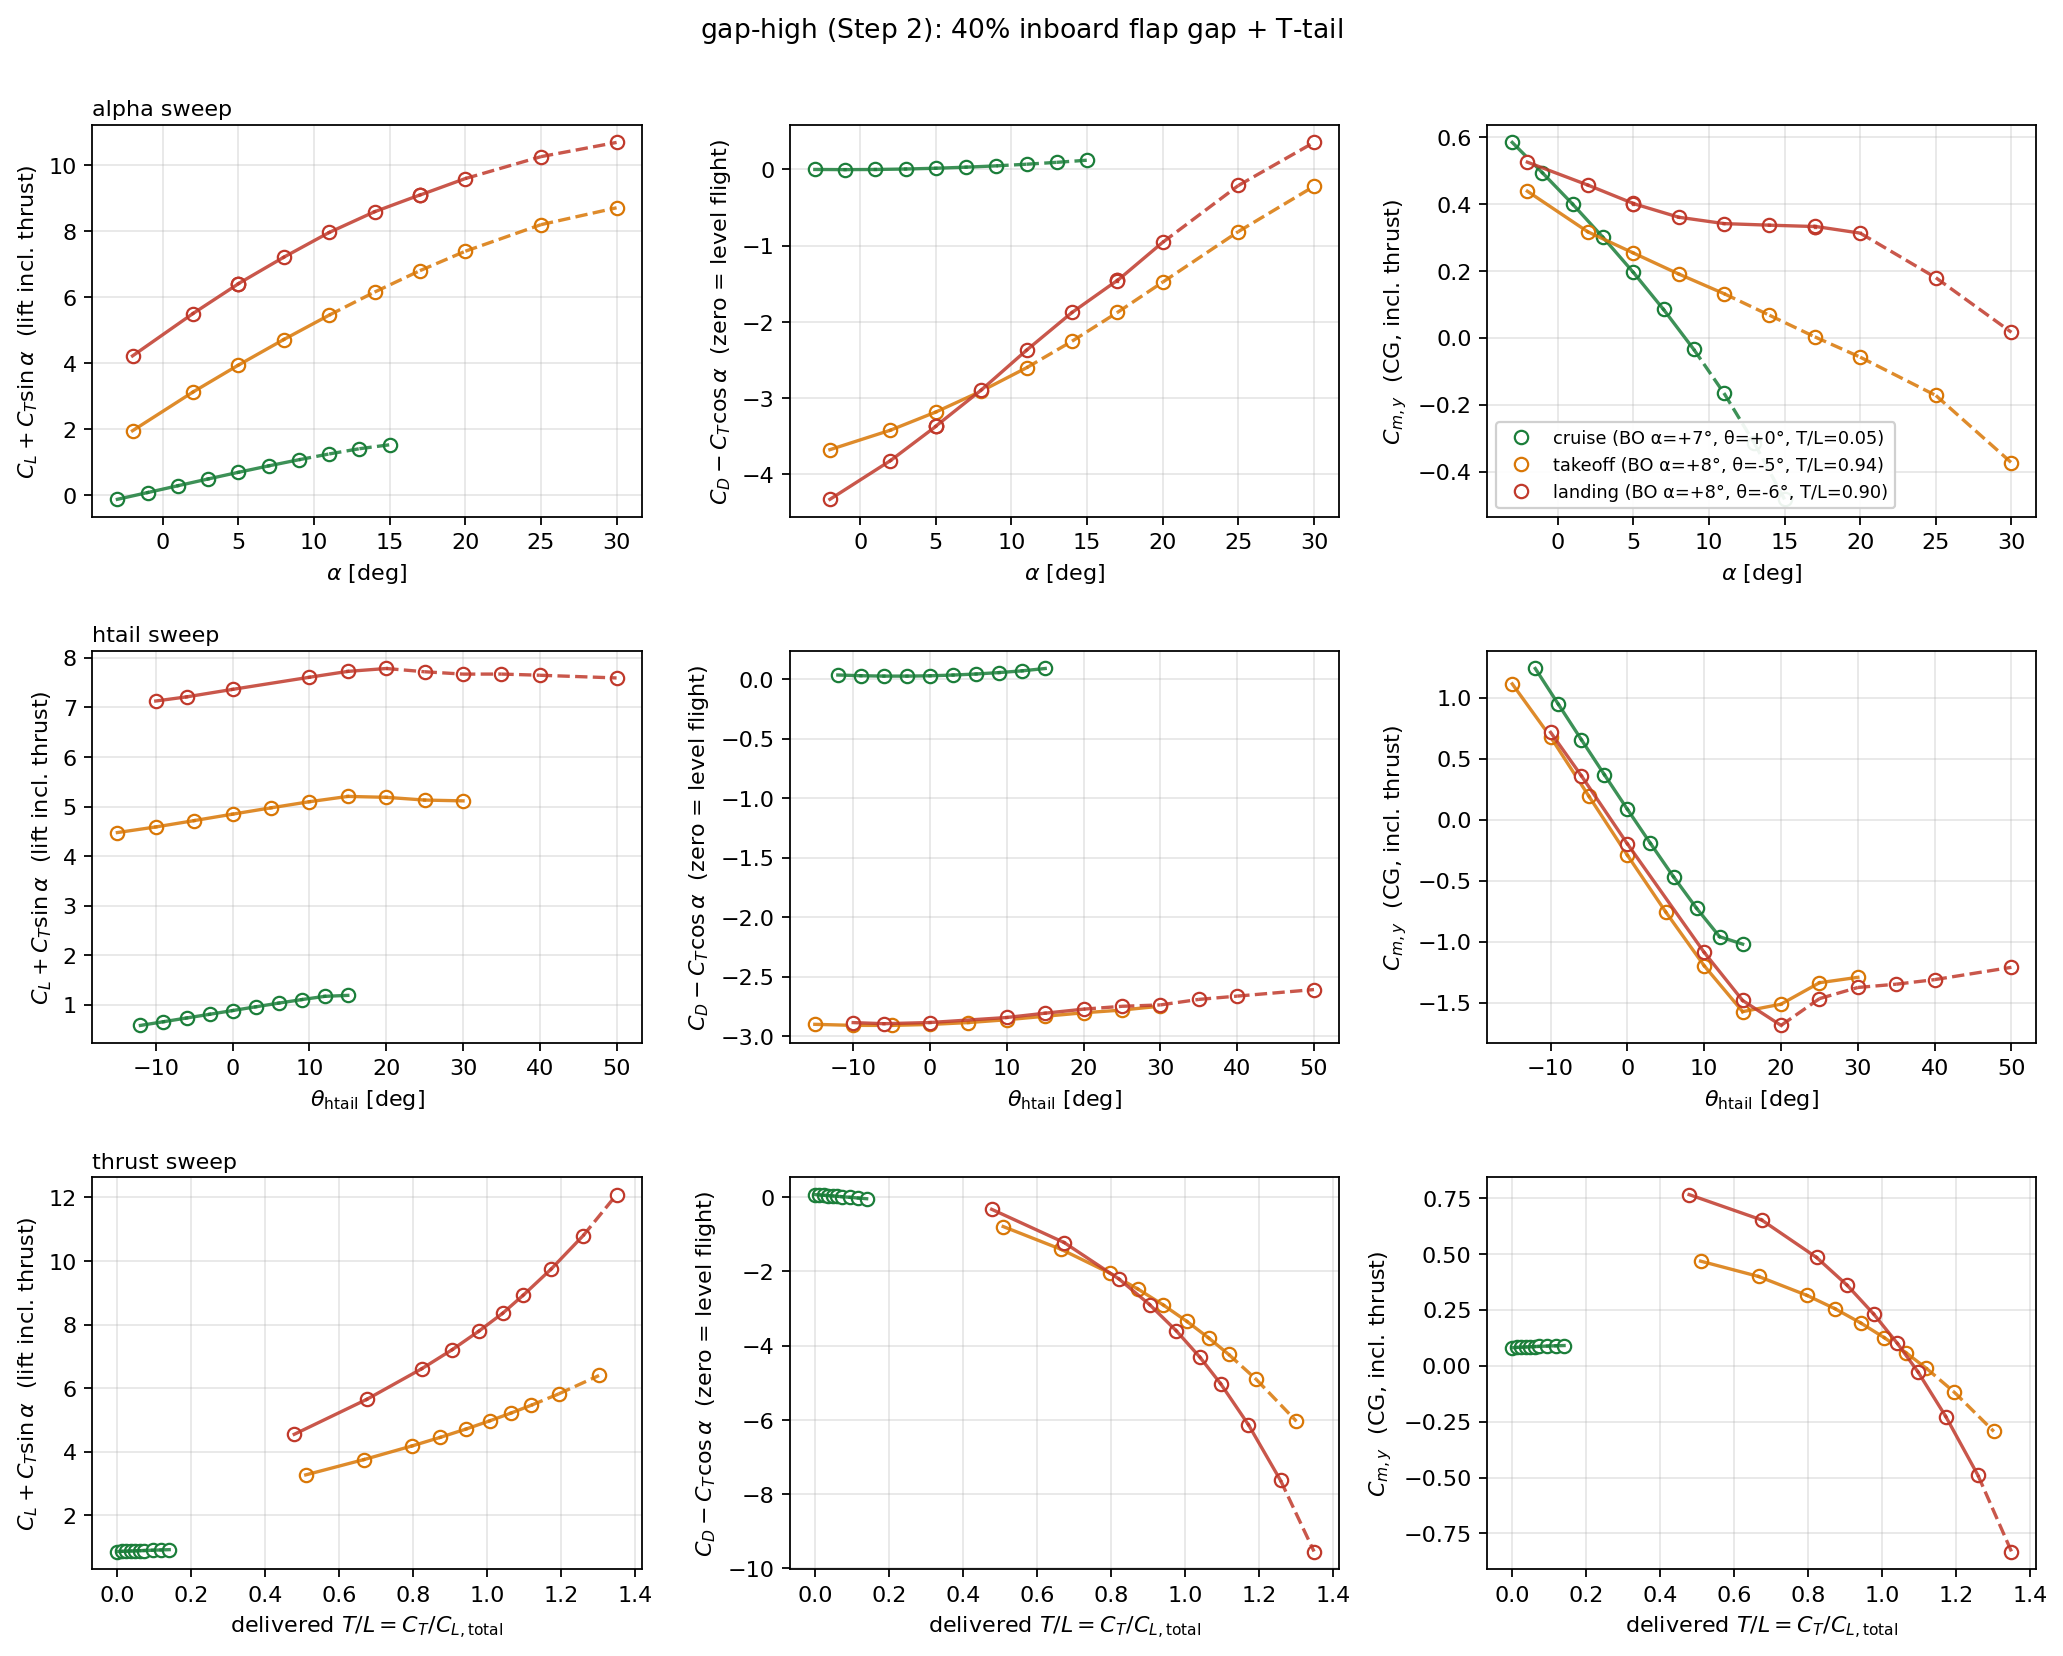
\includegraphics[width=\linewidth]{figures/gap_high_combined_sens.png}
  \caption{Sensitivity sweeps for the gap-high configuration
           (Step~2).  Same axes, color encoding, and
           $C_{L,\mathrm{total}}$/$C_{D,\mathrm{total}}$
           convention as Fig.~\ref{fig:cont-high-sens}.  Compared
           with the cont-high baseline, the flap gap stabilises
           takeoff and landing: takeoff goes from weakly stable to
           moderately stable, and landing flips from mildly
           unstable to weakly stable -- numbers in
           Table~\ref{tab:sm}.  Mechanism: streamwise vortices
           at the flap-segment edges roll the inboard prop wake
           \emph{inboard} along the wing-trailing-edge gap,
           producing a coherent upwash column that impinges on
           the lower surface of the horizontal tail; local
           $d\epsilon/d\alpha$ at the htail station effectively
           flips sign relative to the continuous-flap
           configuration, steepening the htail's restoring
           moment.}
  \label{fig:gap-high-sens}
\end{figure}

The gap costs lie in four predictable channels (reported
qualitatively here): (i) the missing inboard flap drops
landing $C_{L,\max}$ relative to the continuous-flap
configurations, smaller in takeoff where the flap is less
deflected; (ii) the unblown inboard wing loses slipstream
lift augmentation, raising the trimmed approach speed at
fixed weight and thrust -- a real cost for a slow-approach
uSTOL; (iii) the de-blown inboard span sharpens the lift
drop-off at the gap edges and adds two streamwise vortices'
worth of induced drag; (iv) the lower local $C_{L,\max}$ of
the unblown inboard wing biases incipient stall inboard --
the opposite of a benign washout-twisted GA pattern -- which
needs explicit verification in the full paper.  The small
cruise drag improvement (cleaner unflapped central section
vs.\ slightly draggy stowed flap) is real but tiny.

The benefit is the htail-side mechanism evident in
Fig.~\ref{fig:downwash-gap-high}.  Two counter-rotating
streamwise vortices, shed at the gap edges and clearly visible
as $\epsilon$-extrema centred near $y=\pm 2.2\,$m,
$z_\mathrm{body}\approx -1\,$m, roll the inboard prop wake
inward and replace the continuous-flap downwash column with a
centerline \emph{upwash} core.  Reading along the htail dotted
line at $z_\mathrm{body}=+2.63\,$m: $\epsilon$ rises from
$\sim 0^\circ$ at $\alpha=+5^\circ$ to only $\sim +5^\circ$ at
$\alpha=+17^\circ$.  A $12^\circ$ body-$\alpha$ increase
produces just a $\sim 5^\circ$ downwash increase at the htail,
so the htail's effective $\alpha$ rises by $\sim 7^\circ$ --
distinctly more than cont-high's $4$--$5^\circ$ and far above
cont-low's $\sim 2^\circ$.  By the htail-contribution sign
rule this further \emph{stabilises}
$\partial C_{m_{\mathrm{CG}}}/\partial\alpha$, taking landing
$\sm$ from negative to positive and adding margin in takeoff;
the gap is mildly destabilising in cruise where the unflapped
wing sheds no central downwash to invert (Table~\ref{tab:sm}).

\begin{figure}[htb!]
  \centering
  \includegraphics[width=\linewidth]{figures/downwash_gap_high.png}
  \caption{Wind-frame downwash $\epsilon$ at the gap-high
           htail station ($T/L \approx 0.39$),
           $\alpha=+5^\circ$ and $+17^\circ$; same slice and
           conventions as Fig.~\ref{fig:downwash-cont-low}.
           The flap gap replaces the continuous-flap downwash
           column with a centerline \emph{upwash} column
           ($\epsilon < 0$) flanked by two flap-edge vortices.
           The upwash strengthens with $\alpha$ -- the
           $d\epsilon/d\alpha < 0$ that flips the htail
           contribution to $\partial C_{m_{\mathrm{CG}}}/
           \partial\alpha$ from destabilising to stabilising,
           consistent with the landing $\sm$ flip from negative
           to positive in Table~\ref{tab:sm}.}
  \label{fig:downwash-gap-high}
\end{figure}

\subsection{Step 3 -- Ironically, Returning the htail to the Low Position (gap-low)}

With the gap providing the stability fix that the high tail
alone could not, the design optimisation flips.  We are now
free to bring the horizontal tail back \emph{down}.  Ironically
this places the stabiliser at the same vertical position as in
the Step~0 naive baseline -- but now, with the upwash column
from the flap gap providing the stability backbone, the low
position is no longer a liability.  Instead it is a strong
positive: at $z=+0.4\,c_w$ the htail sits inside the merged
10-prop slipstream column.  Locally the htail sees the slipstream
velocity rather than the freestream; at landing thrust
$V_{\mathrm{slip}}/V_\infty \approx 2$--$3$, giving a
$4$--$9\times$ dynamic-pressure boost.  Both
$\partial C_{m_{\mathrm{CG}}}/\partial\alpha$ (stability) and
$\partial C_{m_{\mathrm{CG}}}/\partial\theta_{ht}$ (elevator
authority) scale with local $q$.

\begin{figure}[htb!]
  \centering
  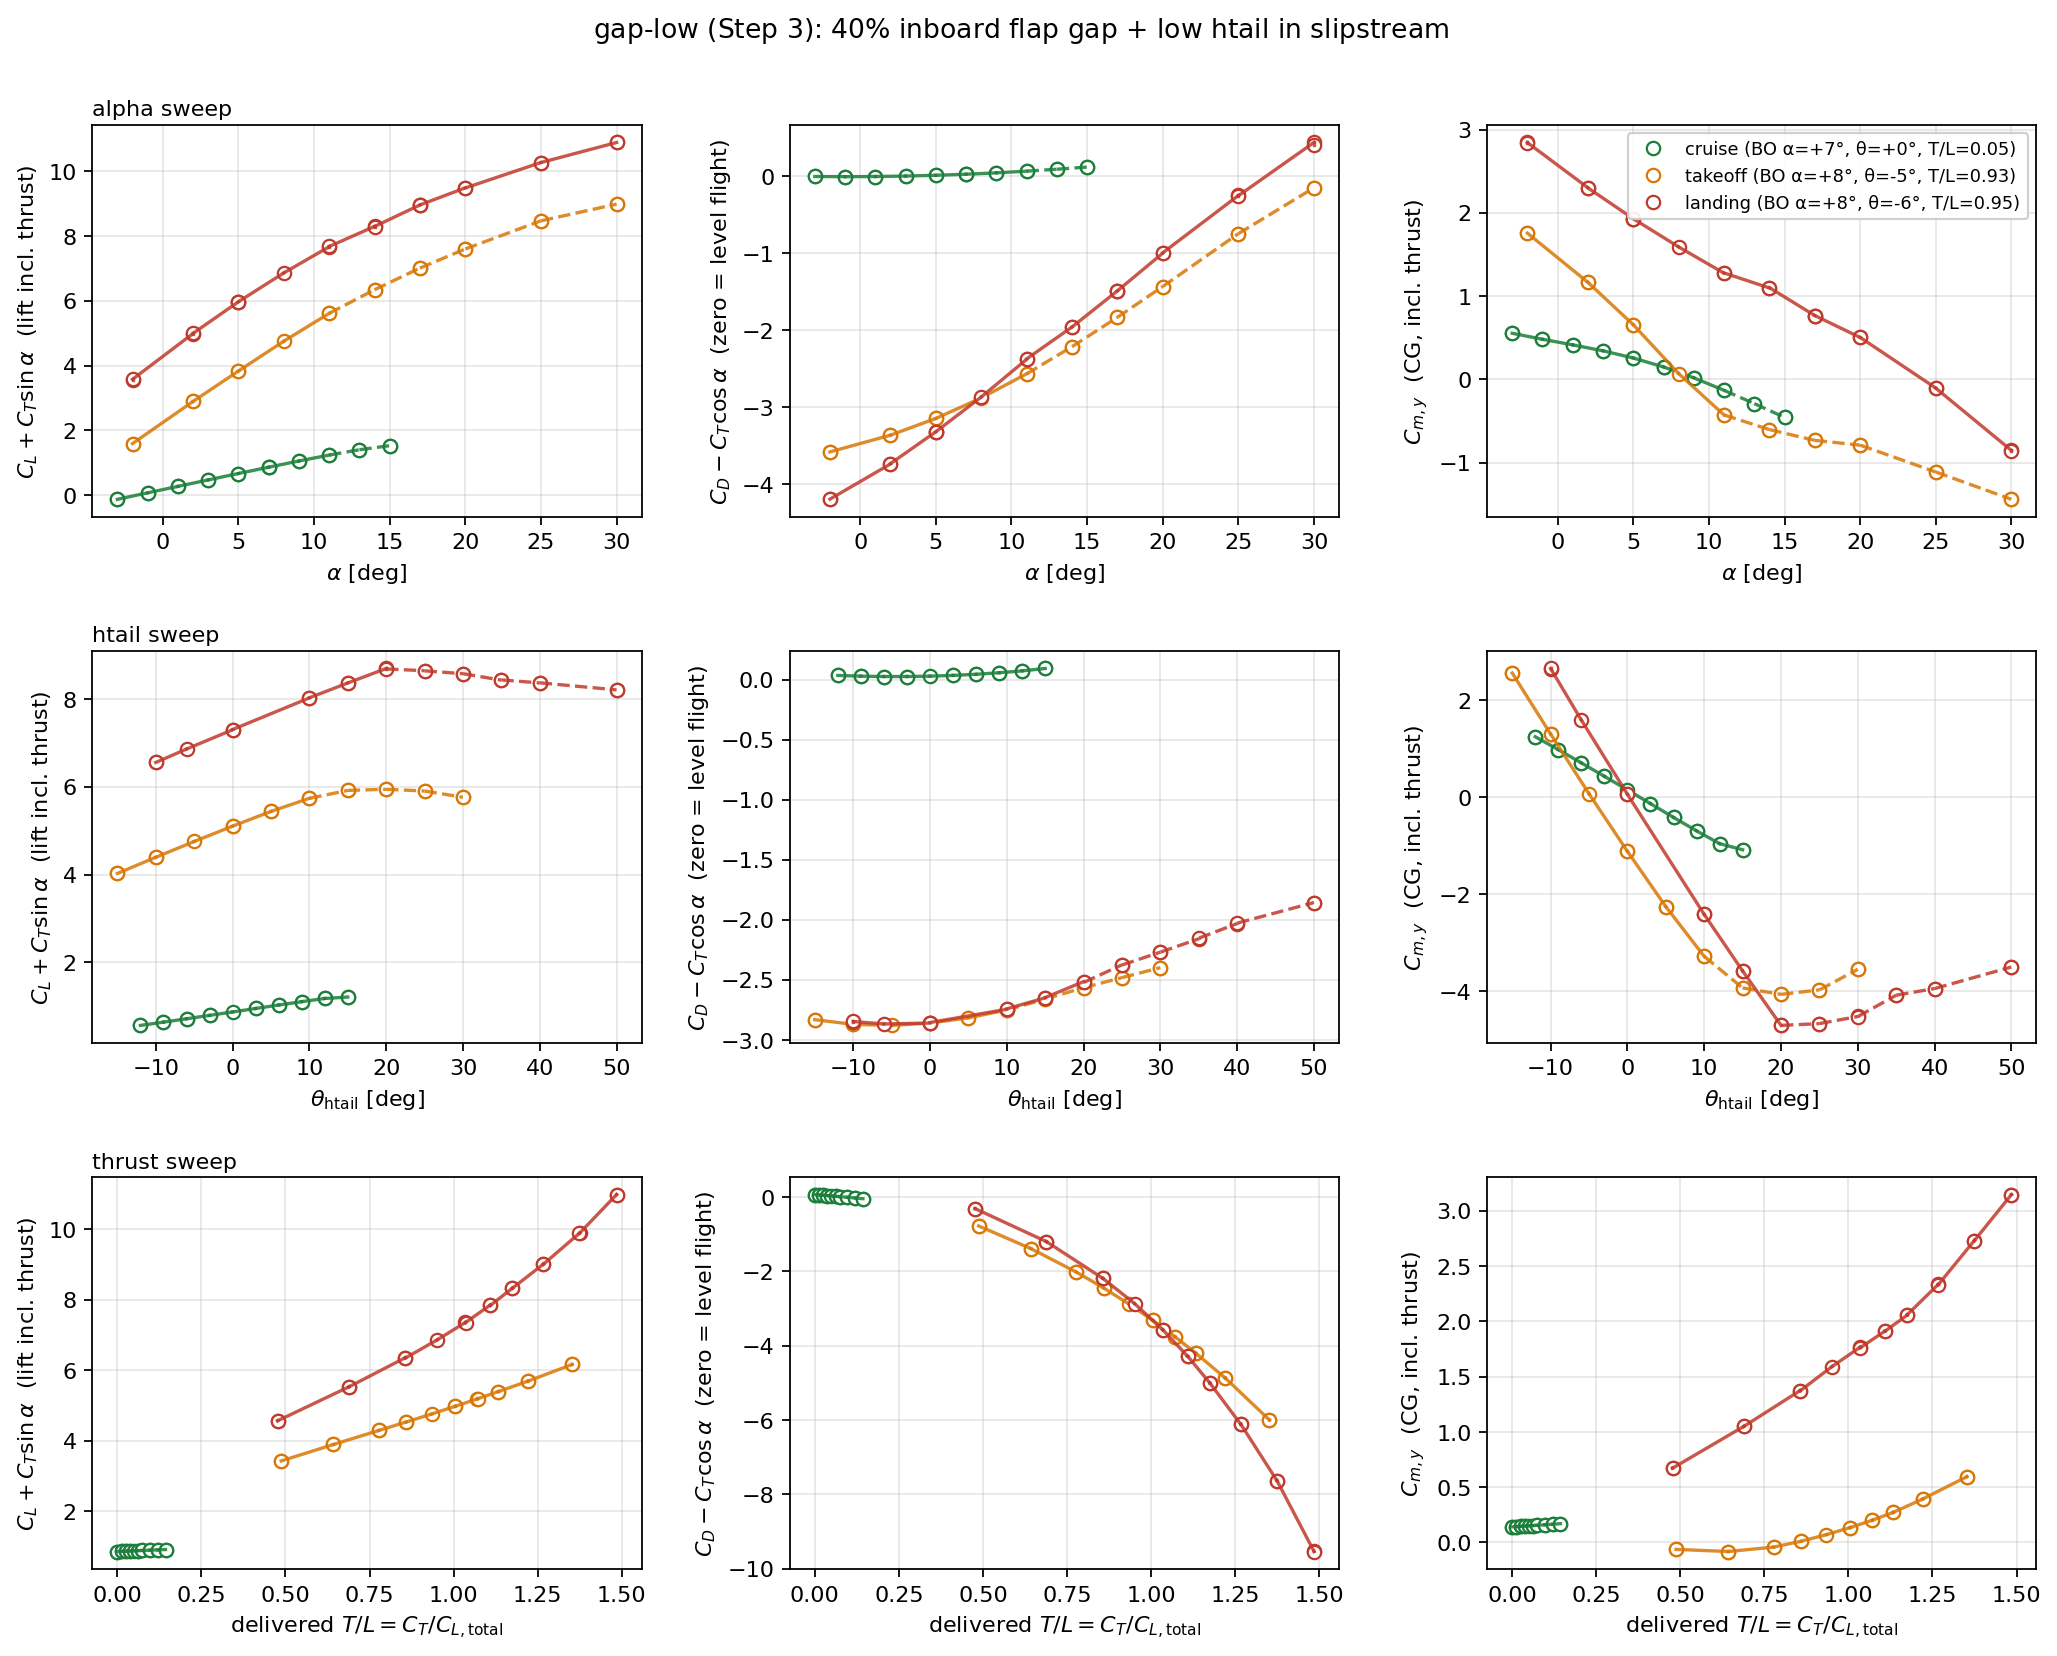
\includegraphics[width=\linewidth]{figures/gap_low_combined_sens.png}
  \caption{Sensitivity sweeps for the gap-low configuration
           (Step~3).  Same axes, color encoding, and
           $C_{L,\mathrm{total}}$/$C_{D,\mathrm{total}}$
           convention as Fig.~\ref{fig:cont-high-sens}.  All
           three phases of gap-low are strongly stable: the
           $C_{m_{\mathrm{CG}}}$-vs-$\alpha$ slopes (third
           column) are sharply negative and the elevator-
           authority slopes
           ($\partial C_{m_{\mathrm{CG}}}/\partial\theta_{ht}$,
           middle row, third column) are roughly doubled
           relative to cont-high.  The htail is in the prop
           slipstream and benefits from a $4$--$9\times$
           dynamic-pressure boost.  Reading $C_{D,\mathrm{total}}$
           in the thrust-sweep row (bottom-middle) gives a
           direct visualisation of the level-flight thrust
           setting at each phase: the $C_{D,\mathrm{total}}=0$
           crossing identifies the trimmed level-flight
           thrust setting at that phase's airspeed.}
  \label{fig:gap-low-sens}
\end{figure}

\begin{table}[htb!]
\centering
\caption{Static margin by configuration and phase, from
         refreshed CFD sensitivity fits with stalled-point
         masks applied.  cont-low and cont-high takeoff and
         landing fits use the $\alpha$-sweep at $\theta_{ht}=+10^\circ$
         (takeoff) / $+20^\circ$ (landing) to keep the htail in
         its linear regime; the BO $\alpha$-sweep at the much lower
         $\theta_{ht}=-5^\circ/-6^\circ$ was contaminated by
         htail stall at high $\alpha$ and produced
         significantly more negative apparent static margins
         (e.g.\ cont-low landing $-29.7\%$ vs the unstalled
         value $-19.5\%$).  Negative $\sm$ indicates instability.}
\label{tab:sm}
\begin{tabular}{lccc}
\toprule
Configuration & Cruise $\sm$ & Takeoff $\sm$ & Landing $\sm$ \\
\midrule
\textbf{cont-low (Step 0; X-57-class)}  & $+46.7\%$ & $+2.9\%$ & $-19.5\%$ \\
cont-high (Step 1; T-tail, continuous flap) & $+55.4\%$ & $+4.8\%$ & $-4.6\%$ \\
gap-high (Step 2; T-tail, $40\%$ flap gap) & $+51.5\%$ & $+12.1\%$ & $+6.4\%$ \\
\textbf{gap-low (Step 3; gap + slipstream)} & $\mathbf{+48.6\%}$ & $\mathbf{+73.1\%}$ & $\mathbf{+91.6\%}$ \\
\textbf{v3 (Step 4; gap-low + short boom)} & $\mathbf{+14.9\%}$ & $\mathbf{+19.0\%}$ & $\mathbf{+21.4\%}$ \\
\bottomrule
\end{tabular}
\end{table}

The gap-low headline numbers (Table~\ref{tab:sm}) are
strongly stable in every phase.  Elevator authority roughly
doubles relative to cont-high in takeoff and landing, exactly
as expected for a $\sim 2\times$ velocity boost on the htail.

The downwash field at the gap-low htail station,
Figure~\ref{fig:downwash-gap-low}, combines the two
mechanisms.  The htail is back at low $z_\mathrm{body}$ -- the
same geometric station that buried it in cont-low -- but the
local flow is qualitatively inverted: the centerline
gap-upwash column still reaches the lower htail position,
while the slipstream column accelerates local $u_\mathrm{world}$
to roughly twice freestream (visible as compressed
iso-$\epsilon$ lines relative to cont-low at matched
$\alpha$).  Reading along the htail dotted line, the
$d\epsilon/d\alpha$ benefit at the low station is somewhat
weaker than at the gap-high T-tail position (the inboard
gap-edge vortices are farther from the low htail vertically),
but the slipstream-doubled local dynamic pressure dominates
the htail-contribution arithmetic: the htail's restoring
moment per degree of effective $\alpha$ scales with
$\eta_t = q_{ht}/q_\infty \approx 4$, and that is the
mechanism behind the Table~\ref{tab:sm} jump to strongly
stable in every flapped phase.  Both pieces -- the gap-induced
$d\epsilon/d\alpha$ flip and the slipstream $q$-boost --
carry over to v3 (Step~4).

\begin{figure}[htb!]
  \centering
  \includegraphics[width=\linewidth]{figures/downwash_gap_low.png}
  \caption{Wind-frame downwash $\epsilon$ at the gap-low
           htail station, $\alpha=+5^\circ$ and $+17^\circ$;
           same slice and conventions as
           Fig.~\ref{fig:downwash-cont-low}.  The low htail
           position is recovered ironically: the gap-upwash
           column reaches the htail span, and the slipstream
           column lifts local $u_\mathrm{world}$ to
           $\approx 2\,V_\infty$.  Combined, these give the
           large-margin landing $\sm$ and the $\approx 2\times$
           elevator-authority boost in Table~\ref{tab:sm}.}
  \label{fig:downwash-gap-low}
\end{figure}

\subsection{Step 4 -- Shortening the Tail Boom (v3)}

The gap-low landing $\sm = +91.6\%$ MAC is unusually stiff
for a piloted aircraft -- roughly an order of magnitude above
a typical GA tail-volume margin.  This headroom is real, and
inviting to spend.  Three structural levers reduce it back
toward a more conventional range while preserving the
gap-induced stability mechanism: (i) reduce the htail span,
(ii) reduce the htail chord, or (iii) shorten the tail boom.
Each cuts the htail's contribution to
$\partial C_{m_{\mathrm{CG}}}/\partial\alpha$, and each carries
a different secondary cost.  Span reduction is the most
risky: it shrinks the htail's exposure to the
slipstream-doubled local dynamic pressure, and -- more
importantly -- it concentrates the remaining htail span over
fewer of the four inboard centerline blowers, so loss of one
inboard propeller punches a larger fractional dead-air hole
in the htail's effective $q$.  Chord reduction trades
nominal-flight stability cleanly against weight and structural
depth and is the most benign on prop-out scenarios.  Boom
shortening pays in pitch-stability arm-length but \emph{gains}
in landing-flare clearance and pilot-input sensitivity (see
Sec.~\ref{sec:envelope} and the flare-geometry argument in
Sec.~3).  All three are worth investigating; this abstract
restricts attention to boom shortening (v3 below) because it
is the most architecturally distinctive and because the
flare-geometry consequences are unique to that lever.  A
practical preliminary design would likely combine boom
shortening with a modest chord reduction; the full paper will
revisit the design matrix on that basis.

v3 retains the gap-low planform but moves the htail
aerodynamic centre from $+3.75\,c_w$ to $+2.0\,c_w$ aft of the
CG (from $\sim 4\,c$ aft of the wing LE to $\sim 2\,c$ aft of
the wing TE), holding $z=+0.4\,c_w$ to stay inside the
slipstream column.  This is the principal configurational
contribution of this paper and is analysed in the next
section.

%====================================================================
\section{Analysis of the v3 Configuration}
%====================================================================

v3 halves the htail moment arm
($k=L_{ht}^{(v3)}/L_{ht}^{(v2)}=2.0/3.75\approx 0.53$) while
retaining the gap-low planform and high-lift system.  The
htail's $\partial C_{m_{\mathrm{CG}}}/\partial\alpha$ and
$\partial C_{m_{\mathrm{CG}}}/\partial\theta_{ht}$ scale
linearly with the moment arm; wing and flap contributions do
not.  The v3 CFD campaign ($3\times(1+19)$ cases) is in flight
with partial coverage (landing $7/20$, takeoff $5/20$, cruise
queueing).  BO trims sit at the low-slow-pass frontier
($\alpha=+15^\circ,\theta_{ht}=-5^\circ$ takeoff;
$\alpha=+25^\circ,\theta_{ht}=+5^\circ$ landing) to probe the
short boom under the most demanding tail-authority condition
(Fig.~\ref{fig:v3-sens}).

\begin{figure}[htb!]
  \centering
  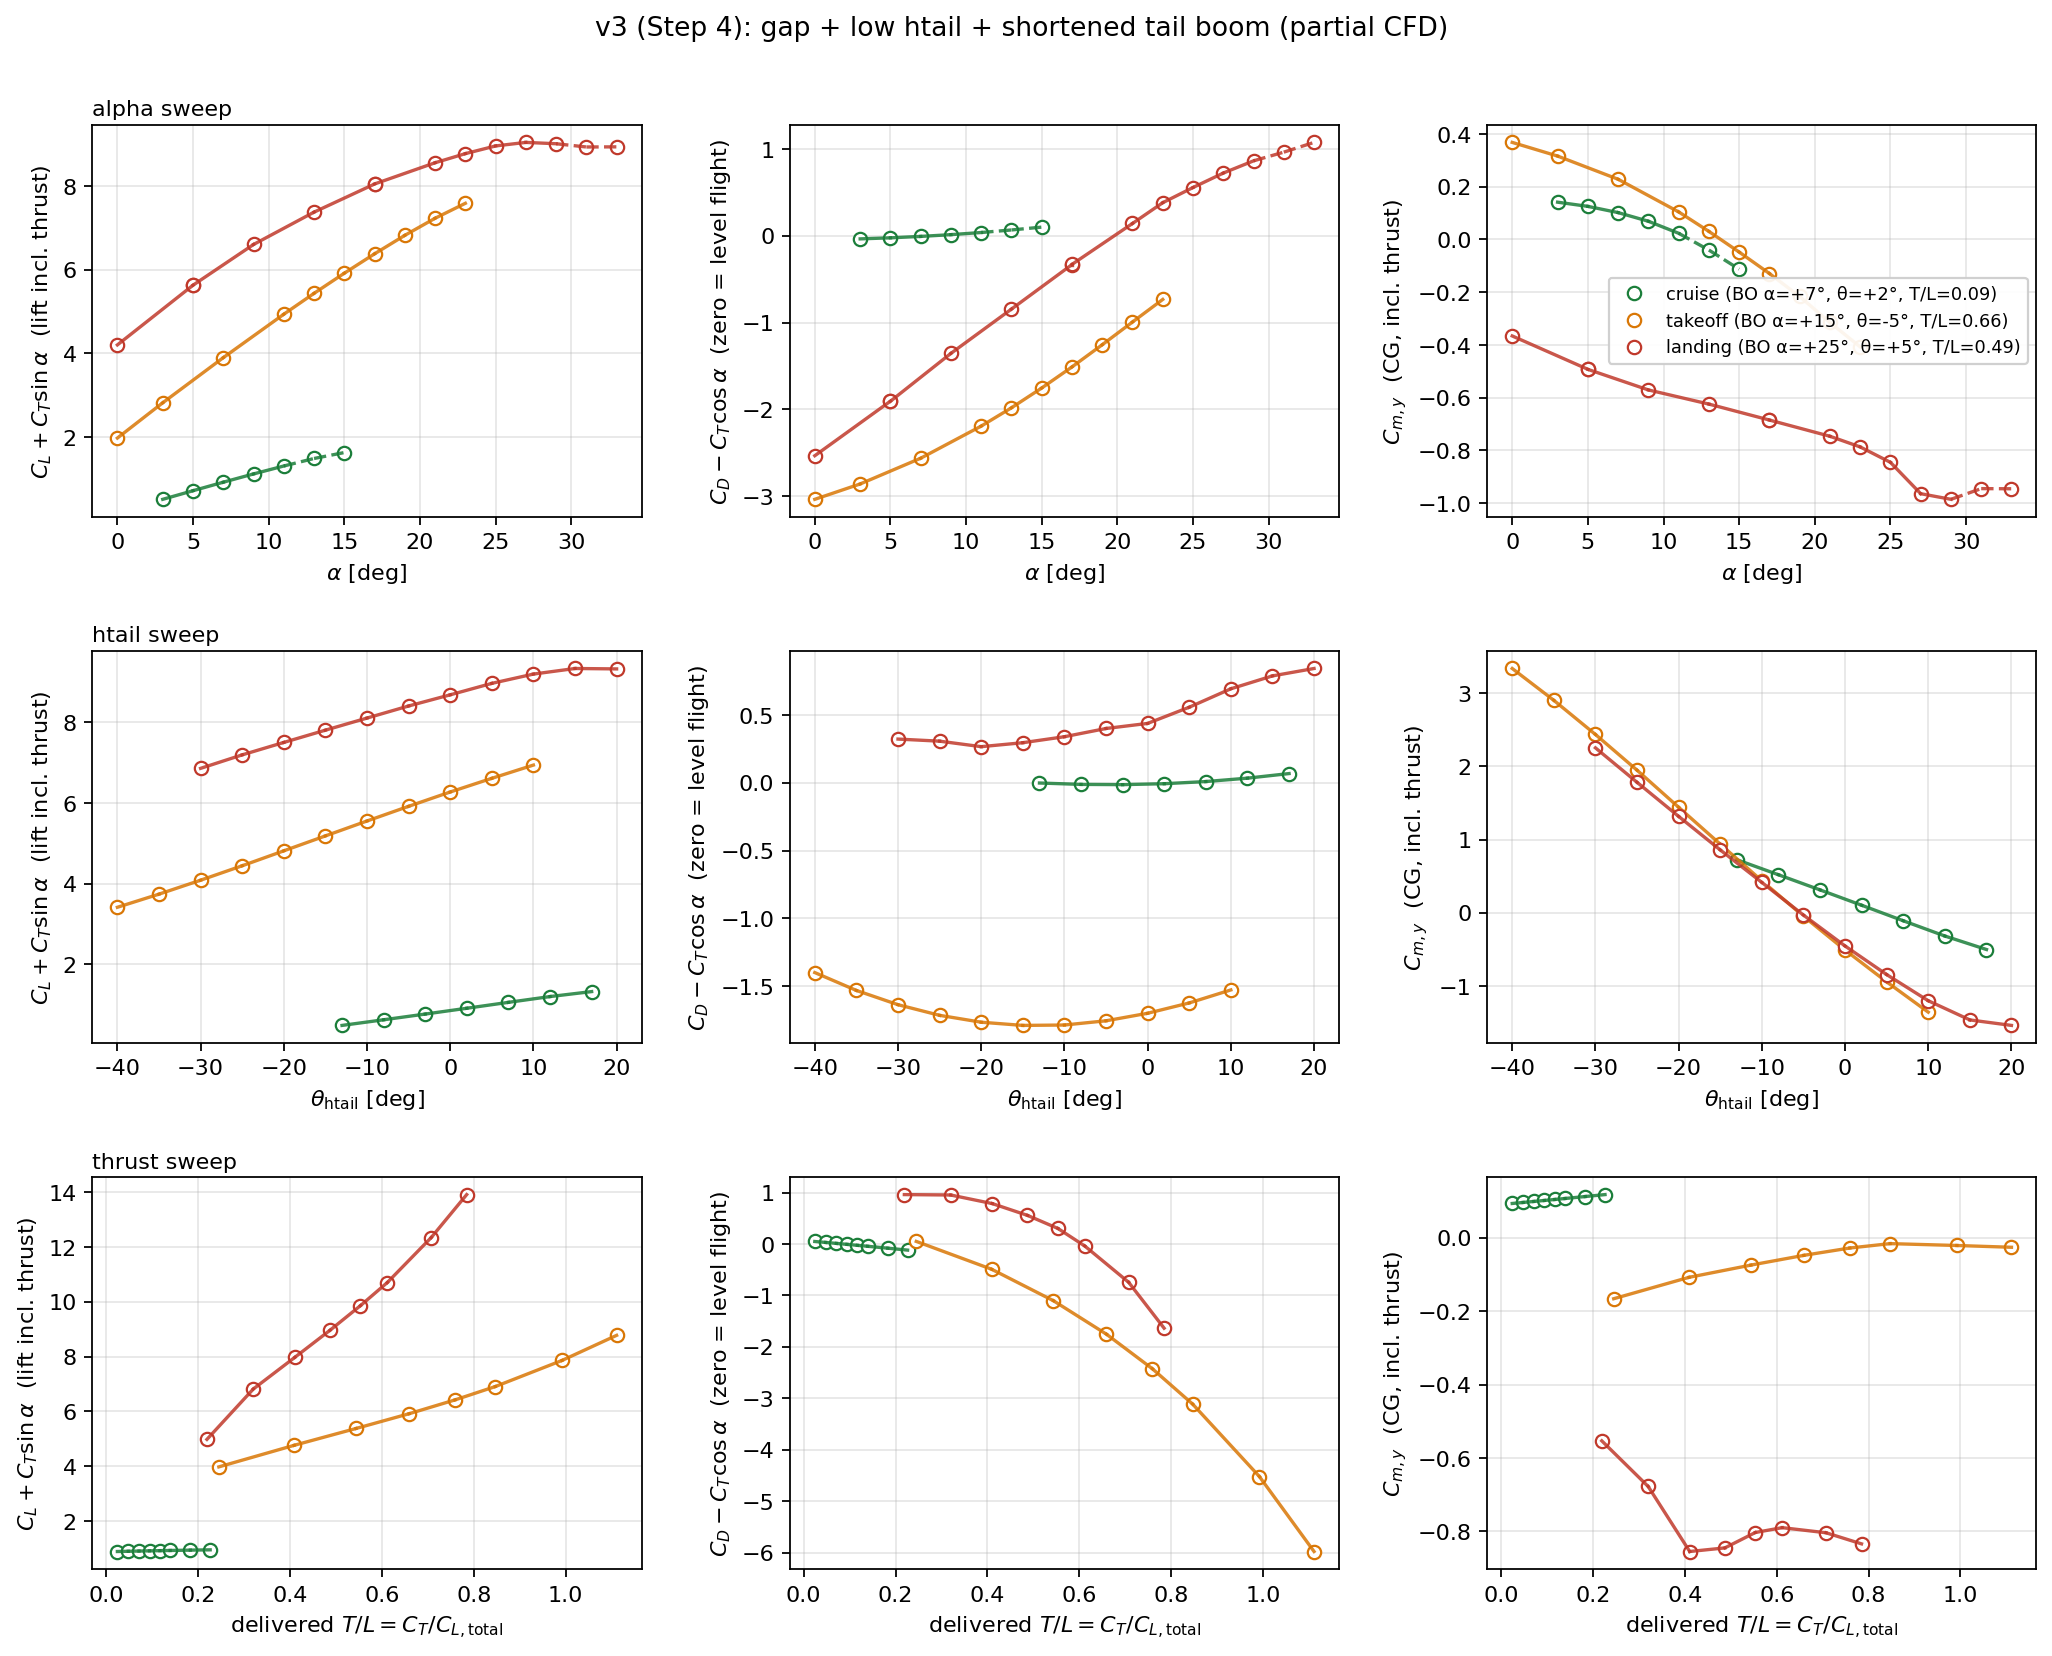
\includegraphics[width=\linewidth]{figures/v3_combined_sens.png}
  \caption{v3 (Step 4) sensitivity sweeps; cruise/takeoff/landing
           rows show the points completed at submission.}
  \label{fig:v3-sens}
\end{figure}

Figure~\ref{fig:downwash-v3} shows $\epsilon$ on the
v3-specific yz-slice ($x_b=$ htail LE $-0.23\,$m).  The
gap-upwash and slipstream-acceleration features of gap-low are
preserved at the v3 station; the htail span sits inside the
upwashed, accelerated column.  This is the geometric basis for
v3 retaining usable stability and
elevator authority despite the $\sim 47\%$ moment-arm
reduction.

\begin{figure}[htb!]
  \centering
  \includegraphics[width=\linewidth]{figures/downwash_v3.png}
  \caption{Wind-frame downwash $\epsilon$ at the v3 htail
           station ($x_b=$ htail LE $-0.23\,$m, v3 BO landing
           trim), $\alpha=+5^\circ$ and $+17^\circ$; conventions
           as Fig.~\ref{fig:downwash-cont-low}.  The shortened
           boom retains the gap-upwash column and the
           slipstream acceleration at the htail station;
           combined with the $0.53\times$ moment arm this
           gives the v3 trim headroom of Fig.~\ref{fig:v3-sens}.}
  \label{fig:downwash-v3}
\end{figure}

\subsection{Trimmable flight envelope}
\label{sec:envelope}

To read off what the configuration can \emph{do}, we march
through an $(\alpha, T/L)$ grid: at each point we pick
$\theta_{ht}$ to trim the moment, evaluate $C_L$, $C_D$,
$C_{T,\mathrm{del}}$ from local linear sensitivities, and solve
the Newtonian force-balance for equilibrium $V$ and $\gamma$.
The table is generated from the \emph{partial v3 short-boom}
CFD sensitivities currently on hand
(\texttt{post/v3/plot\_*\_sensitivities.py}), centred on the
v3 BO trim points ($\alpha=+7/+15/+25^\circ$ in
cruise/takeoff/landing) and spanning the low-slow-pass
envelope.  Final numbers refresh when the remaining v3 sweep
points land.

\begin{table}[htb!]
\centering
\small
\caption{\textbf{Trimmable flight envelope, v3 short-boom}.  At
         each $(\alpha, T/L)$ grid point, $\theta_{ht}$ trims
         the moment; equilibrium $V$ and $\gamma$ follow from
         the Newtonian force balance with delivered actuator-
         disk thrust held constant.  $T/L$ is the delivered
         thrust-to-total-lift ratio at the trimmed airspeed.
         Highest-$T_{\mathrm{mult}}$ entries at takeoff
         $\alpha=+12^\circ$ and $+15^\circ$ are omitted: there
         the drag balance admits no real positive $V$ root
         (delivered thrust exceeds the largest steady-flight
         drag at any airspeed), i.e.\ those points are not
         steady-flight operating conditions.  Slopes from
         \texttt{post/out/v3/*\_sweep\_data.csv}; table
         generated by \texttt{post/v3/equilibrium\_grid.py}.}
\label{tab:v3-envelope}
\begin{tabular}{ccccccc}
\toprule
Phase & $\alpha$ [deg] & $T/L$ & $\theta_{ht}$ [deg]
   & $C_L$  & $V$ [kt] & $\gamma$ [deg] \\
\midrule
\multirow{9}{*}{Cruise}
  & $+5$ & $0.05$ & $+5.04$ & $0.79$ & $92.3$ & $-1.8$  \\
  & $+5$ & $0.09$ & $+5.16$ & $0.80$ & $91.5$ & $+0.5$  \\
  & $+5$ & $0.14$ & $+5.28$ & $0.81$ & $90.6$ & $+2.9$  \\
  & $+7$ & $0.05$ & $+4.33$ & $0.96$ & $83.3$ & $-2.0$  \\
  & $+7$ & $0.09$ & $+4.45$ & $0.97$ & $82.6$ & $+0.5$  \\
  & $+7$ & $0.14$ & $+4.57$ & $0.98$ & $81.9$ & $+2.9$  \\
  & $+9$ & $0.05$ & $+3.62$ & $1.14$ & $76.5$ & $-2.1$  \\
  & $+9$ & $0.09$ & $+3.74$ & $1.15$ & $75.9$ & $+0.4$  \\
  & $+9$ & $0.14$ & $+3.86$ & $1.16$ & $75.2$ & $+2.9$  \\
\midrule
\multirow{7}{*}{Takeoff}
  & $+9$  & $0.37$ & $-3.64$ & $3.42$ & $42.9$ & $+5.9$  \\
  & $+9$  & $0.75$ & $-3.37$ & $3.93$ & $37.2$ & $+22.9$ \\
  & $+9$  & $2.54$ & $-3.10$ & $4.44$ & $22.6$ & $+60.1$ \\
  & $+12$ & $0.37$ & $-4.71$ & $3.88$ & $39.9$ & $+4.1$  \\
  & $+12$ & $0.76$ & $-4.44$ & $4.39$ & $34.5$ & $+22.2$ \\
  & $+15$ & $0.37$ & $-5.78$ & $4.34$ & $37.3$ & $+2.8$  \\
  & $+15$ & $0.78$ & $-5.51$ & $4.86$ & $32.2$ & $+21.7$ \\
\midrule
\multirow{9}{*}{Landing}
  & $+15$ & $0.22$ & $-2.70$ & $4.97$ & $35.3$ & $-10.9$ \\
  & $+15$ & $0.40$ & $-3.18$ & $5.83$ & $31.9$ & $-7.1$  \\
  & $+15$ & $0.58$ & $-3.66$ & $6.70$ & $29.1$ & $-0.8$  \\
  & $+20$ & $0.23$ & $-3.94$ & $5.36$ & $33.4$ & $-13.5$ \\
  & $+20$ & $0.40$ & $-4.42$ & $6.23$ & $30.2$ & $-8.4$  \\
  & $+20$ & $0.58$ & $-4.90$ & $7.10$ & $27.4$ & $-1.0$  \\
  & $+25$ & $0.23$ & $-5.18$ & $5.76$ & $31.7$ & $-15.7$ \\
  & $+25$ & $0.40$ & $-5.66$ & $6.63$ & $28.6$ & $-9.6$  \\
  & $+25$ & $0.60$ & $-6.13$ & $7.50$ & $25.8$ & $-1.2$  \\
\bottomrule
\end{tabular}
\end{table}

In cruise ($\alpha\in[+5,+9]^\circ$) the aircraft trims with
$\theta_{ht}\in[+3.6,+5.3]^\circ$, modest deflections inside
the htail's unstalled range, with $|\gamma|\lesssim 3^\circ$
and $V\in[75,92]\,$kt across the cruise-thrust grid.  In
takeoff ($\alpha\in[+9,+15]^\circ$, $T/L\in[0.37,0.78]$) trim
$\theta_{ht}$ is mildly negative everywhere ($\le 0^\circ$,
inside the $+12^\circ$ stall margin); $\gamma$ runs from a
mild $+3$--$+6^\circ$ climb at $T/L\approx 0.37$ to a steep
$+22^\circ$ blown-lift climb at $T/L\approx 0.77$, with
$V\in[23,43]\,$kt throughout.  In landing
($\alpha\in[+15,+25]^\circ$) approach is steep at low thrust
($\gamma\in[-11,-16]^\circ$ at $T/L\approx 0.22$), shallower
at mid-thrust ($-7$ to $-10^\circ$), and near-level at
high-thrust ($\gamma\approx -1^\circ$, a power-on go-around
margin); $V\in[26,35]\,$kt and the maximum trim magnitude
$|\theta_{ht}|=6.1^\circ$ sits comfortably inside the
$+20^\circ$ landing stall margin.  The v3 design target --
$\alpha\approx +25^\circ$, $T/L\approx 0.4$,
$\gamma\approx -10^\circ$, $V\approx 29\,$kt -- sits squarely
inside the grid.

\subsection{Slipstream coverage at the shorter arm}

The merged 10-prop slipstream column spreads from
$z\in[-0.3,+0.6]\,c_w$ at the v2 htail station
($4.4\,c_w$ downstream of the disks) to a slightly tighter
$z\in[-0.2,+0.55]\,c_w$ at the v3 station
($2.7\,c_w$ downstream).  The v3 htail at $z=+0.4\,c_w$ sits
comfortably inside this band; moving it up by more than
$\sim 0.1\,c_w$ would risk exiting the upper edge, which is
why v3 retains the v2 low-tail vertical position.

\subsection{Geometric benefits at landing flare}

Rotating about the main-gear contact at
$(x_g,z_g)=(+0.50,-1.00)\,c_w$ maps a body-frame point
$(x,z)$ to $z'=z_g-(x-x_g)\sin\theta+(z-z_g)\cos\theta$.  For
the htail TE at $z=+0.4\,c_w$ and a $30^\circ$ flare attitude
this gives $z'_{TE}=-1.79\,c_w$ for v2 ($x_{TE}=+4.5\,c_w$,
$0.79\,c_w$ below ground -- tail strike) versus
$z'_{TE}=-0.79\,c_w$ for v3 ($x_{TE}=+2.5\,c_w$,
$0.21\,c_w$ of clearance).  At a conventional $17^\circ$
flare v2 is still marginal ($0.17\,c_w$ below ground) while
v3 is easy ($0.75\,c_w$ above).  The v3 short boom therefore
supports the uSTOL low-slow-pass landing
($\alpha\approx +30^\circ$ at $\gamma=0$ in ground effect,
$V\lesssim 20\,$kt) -- one row beyond the bottom of
Table~\ref{tab:v3-envelope}, a target the in-progress v3
sweep extension is configured to probe directly.

\subsection{Cautions and CFD validation plan}

The partial v3 CFD sweep reported here (Table~\ref{tab:sm})
gives measured static margins of $+15/+19/+21\%$ MAC across
cruise/takeoff/landing -- significantly smaller than the
simple-arm-scaling linear projection ($\sim 0.53\times$ of the
v2 gap-low slopes would have predicted $+26/+39/+49\%$ MAC).
The shortfall is consistent with the known steepening of the
wing-wake downwash gradient at the htail station as the htail
moves closer to the wing: for flapped-wing configurations this
effect typically reduces the effective
$\partial C_{m_{\mathrm{CG}}}/\partial\alpha$ contribution of
the htail by $15$--$25\%$ beyond simple arm-scaling, and an
additional reduction of similar magnitude is plausible from the
short boom changing the local downwash field structure.  All
three v3 phases remain strongly stable at these reduced margins.
Completion of the v3 CFD campaign (full $1+19$ sweep per phase)
is in flight and will sharpen these values for the full paper.

\paragraph{Asymmetric prop-out under the short boom.}
The $47\%$ shorter boom also shortens the vertical-tail yaw
arm, weakening rudder recovery from asymmetric thrust loss.
Four of the ten disks sit on the inboard gap region and blow
directly toward the empennage, so the rudder stays inside an
energised slipstream after one or two \emph{outboard} disks
fail.  What the geometry does \emph{not} protect against is a
simultaneous loss of one of these four centerline blowers at
low airspeed: the gap-low/v3 upwash column that anchors pitch
stability is itself partially de-energised, and the short boom
no longer has the lever arm to recover.  We anticipate v3
will require an eSTOL height-velocity (``dead man's curve'')
exclusion region in $(V, h_{\mathrm{AGL}})$ -- not a defect
unique to v3, but amplified enough by the short boom that it
must be characterised rather than assumed small.

\paragraph{Actuator-disk methodology limitations.}
The uniform-pressure-jump actuator disk captures the
time-averaged axial thrust and slipstream tube but omits prop
swirl and discrete helical tip vortices.  Swirl is the concern
here: the gap-low/v3 story relies on a \emph{symmetric}
centerline upwash column from the flap-gap edge vortices, and
an inboard-prop swirl component of the same handedness as one
edge vortex (and opposite the other) could deflect the column
off-centre.  A swirl-augmented disk or a rotor-resolving
sliding-mesh spot-check at the v3 landing trim point
(Sec.~\ref{sec:expected}) is needed to bound the error; the
asymmetric prop-out cases above are the most likely regime for
actuator-disk and rotor-resolving predictions to diverge.

%====================================================================
\section{CFD-Based Dynamic Maneuver Simulation}
\label{sec:dynamic}
%====================================================================

Steady CFD with the rigid body fixed underpins
Secs.~\ref{sec:evolution}--\ref{sec:envelope}, but the eventual
target is a \emph{dynamic} landing flare with the ground plane.
We have built and exercised a CFD-coupled 6-DOF longitudinal
framework on a v3 cruise phugoid as a stepping stone so the
flare simulation can be set up with confidence.

\subsection{Method: nested rotation zones + UDD 6-DOF}

Flow360 couples CFD to user dynamics through (i) rotation volume
zones (sliding-mesh interfaces about an axis) and (ii) the
User-Defined-Dynamics (UDD) block, which computes a state from
integrated forces and moments and feeds the rotation-zone
angles via \texttt{FromUserDefinedDynamics}.  We chain four
nested rotation cylinders in a robot-arm topology
(Fig.~\ref{fig:phugoid-setup}): an outer 2-link arm
(\emph{shoulder} + \emph{elbow}, $L_1=L_2=750\,c_w$) translates
the airframe through the workspace; inner cylinders rotate the
airframe about its CG and the htail about its pivot.  Each
physical step the UDD reads the airframe wall force
$(F_x, F_z, M_y)$, integrates
$\dot V_x=F_x/m + T_{\mathrm{disk}}/m$,
$\dot V_z=F_z/m - g$, $\dot q=M_{y,\mathrm{CG}}/I_{yy}$
(plus kinematics), and inverse-kinematics-resolves the
shoulder/elbow angles so the airframe lands at $(x_{cg},z_{cg})$.
The disk thrust enters separately because it is a volume body
force.  The moment is translated from a fixed world-frame
moment centre to the current CG via
$M_{y,\mathrm{CG}}=M_{y,\mathrm{mc}}+(m_z-z_{cg})F_x-
(m_x-x_{cg})F_z$, with the moment centre placed at the
initial-CG world position to minimise lever-arm cancellation.

\begin{figure}[htb!]
  \centering
  \includegraphics[width=\linewidth]{figures/v3_phugoid_setup.png}
  \caption{Four-cylinder robot-arm topology.  Left: world-frame
           workspace overview; freestream is along $+x$ from the
           left edge.  Cyl~1 (shoulder, grey) and cyl~2 (elbow,
           orange) form the translating 2-link arm
           ($L_1=L_2=750\,c_w$); their links are drawn as blue
           and orange line segments; black dots mark joints.
           Right: airframe-scale side view in body frame
           (origin at CG, $+x$ toward tail, $+z$ up).  Solid
           shapes are the geometry meshed in CFD: wing at
           $x\in[-0.5,+0.5]\,c_w$, htail at $[+1.5,+2.5]\,c_w$,
           actuator disk at $x=-0.7\,c_w$.  Dotted contours
           (fuselage belly, landing gear, ground) are schematic
           context not present in the simulation.  Cyl~3
           (airframe-pitch, blue) is a circle of radius
           $2.9\,c_w$ centred at the CG -- visible as two
           near-vertical arcs at $x\approx\pm 2.9\,c_w$.  Cyl~4
           (htail-pitch, magenta) is a circle of radius
           $0.85\,c_w$ centred at the htail $c/4$
           ($x=+1.75\,c_w$), giving a $0.10\,c_w$ design gap
           between htail TE and cyl~4 on the $+x$ side.
           Cyl~2's outer boundary closest to the body lies on
           the nose side, drawn as the orange arc at $x \approx
           -3\,c_w$, $0.10\,c_w$ outside cyl~3 there.  Cyl~1's
           nearest body-frame boundary point is $\sim 313\,c_w$
           off the airframe and cannot be drawn at this scale;
           see the left panel.}
  \label{fig:phugoid-setup}
\end{figure}

\paragraph{Two implementation lessons.}
(i) UDD must read forces from the \emph{last} pseudo-step of
each physical step, not the first; first-step forces are
computed against the previous attitude, giving a $\sim 10\%$
noise floor on $C_{m,\mathrm{CG}}$ that dominates the residual
signal $\sim 100\times$ after moment translation.  (ii) Pseudo
steps per physical step must be large enough for several
decades of residual drop; we use $200$ (vs.\ Flow360 default
$20$--$50$), reaching a $\sim 0.05\%$ noise floor on
$C_{m,\mathrm{mc}}$ -- sufficient to expose $\sim 10^3\,$N$\cdot$m
$M_{y,\mathrm{CG}}$ signals out of $\sim 10^5\,$N$\cdot$m raw
moments.

%====================================================================
\section{Expected Full-Paper Contributions}
\label{sec:expected}
%====================================================================

The full SciTech 2027 manuscript (1 December 2026 deadline)
will extend this extended abstract with:

\begin{itemize}\setlength\itemsep{1pt}
  \item Completion of the v3 and gap-high CFD sweeps (full
        $1+19$ cases per phase), sharpening Table~\ref{tab:sm}
        and Table~\ref{tab:v3-envelope} and isolating
        gap-alone vs.\ $z$-alone contributions through the
        $2\times 2$ matrix.
  \item Common-$(T/L,\theta_{ht})$-grid rerun across all four
        v2 configurations to remove the cross-configuration
        bias of Sec.~\ref{sec:caveats}, and a body-fixed
        downwash slice with explicit frame convention.
  \item Nonlinear phugoid dynamic simulations for cont-high,
        gap-low~v2, and v3 at the landing trim -- damping
        ratio, natural frequency, and step-response time
        histories, converting the static-margin headline into
        handling qualities.
  \item Ground-effect landing flare in CFD: $-3^\circ$
        approach, flare at $h=2\,$ft AGL, throttle chop,
        pitch-up to $+17^\circ$; resolves ground-effect lift
        amplification, real-time htail authority, and
        slipstream--ground interaction.
  \item Asymmetric prop-out sweep + dead-man's-curve
        characterisation: single- and two-disk-out at the
        landing trim, centerline vs.\ outboard cases separated,
        producing the $(V, h_{\mathrm{AGL}})$ exclusion region.
        Crucially, each inner-prop-out case will be evaluated
        for both \emph{stability margin} ($\sm$ refit on the
        de-energised local flow at the htail) and \emph{htail
        stall margin} (recomputed effective $\alpha_{ht}$ now
        that the centerline upwash column is partially
        collapsed) -- both can degrade substantially even when
        the airframe remains trimmable.
  \item Actuator-disk validation: a swirl-augmented disk
        variant and a rotor-resolving sliding-mesh spot-check
        at v3 landing
        \cite{Jia2023RotorFundamentals,Jia2021TiltrotorDES},
        bounding swirl/helical-tip-vortex error on the
        symmetric upwash column.
  \item Acoustic spot-check at design tip-Mach and a gap-fraction
        sensitivity (fixed at $0.40$ here).
  \item Numerical practice for the four-cylinder dynamic-CFD
        framework: meshing strategy across the nested rotation
        zones, residual-convergence behaviour as a function of
        pseudo-steps per physical step, wall-time cost per
        simulated second on the phugoid and the landing-flare
        cases, and the sensitivity of the integrated CG moment
        to the moment-translation cancellation discussed above.
\end{itemize}

\paragraph{Mapping the stability paradox across design space.}
The $2\times 2$ design matrix of \S\ref{sec:evolution} is a
four-point sample of a continuous five-dimensional design
space $(f_{\mathrm{gap}}, z_{ht}, x_{ht}, \alpha, T/L)$.  A
central question this abstract cannot yet answer is whether
the gap-low stability paradox is a finite-volume basin robust
to perturbation along each axis, or a knife-edge that the
$2\times 2$ happens to straddle.  The full paper will recover
the boundary of the paradox region (where the landing $\sm$
crosses zero) via an adaptive-sampling campaign: an AVL
vortex-lattice linear prior, a residual Gaussian-process
correction fit to acquired Flow360 cases, and an acquisition
layer that preferentially queries near sign reversals in
$\partial C_{m_{\mathrm{CG}}}/\partial\alpha$, supplemented by
a compact learned next-point policy trained on synthetic
aerodynamic databases of known ground truth.  The architecture
has been validated on a $2{,}333$-case BET-RANS oracle of the
NASA X-57 Maxwell, recovering a previously unresolved
nonlinear stall transition at $\sim 30$--$45\%$ value-RMSE
improvement over Latin-hypercube sampling at matched budget,
with $|\nabla C_L|$ RMSE $\sim 52\%$ lower than LHS at small
budgets.\footnote{Flexcompute internal study; details to
appear in the full paper.}  Reconstruction quality will be
reported in a Sobolev-type norm
$\|\hat C_{m_{\mathrm{CG}}}-C_{m_{\mathrm{CG}}}^{\star}\|_{H^1}$
on the slope and curvature of $C_{m_{\mathrm{CG}}}$, which is
the engineering-relevant metric for a stability-margin
question and where the adaptive sampler's advantage is
largest.  The campaign is orchestrated end-to-end in
Flexcompute Thread,\footnote{Flexcompute Thread,
\url{https://thread.simulation.cloud}: integrated
data-management framework that unifies the AVL prior,
Flow360 RANS, the residual GP, and the learned next-point
policy as queryable objects of the same design study.} which
also exposes derived engineering quantities (static margin,
sensitivity slopes, Sobolev-norm reconstruction error)
alongside the primitive CFD coefficients.  Deliverables:
(i) the recovered paradox-region boundary surface in the 5-D
space; (ii) Sobolev-norm convergence of reconstructed
$C_{m_{\mathrm{CG}}}$ vs adaptive case count
$N_{\mathrm{adaptive}}$, with the equivalent uniform-grid
budget $N_{\mathrm{uniform}}$ as the comparison anchor; and
(iii) a held-out blind verification point at which the
learned policy predicted the boundary location, used to
demonstrate generalisation outside the training set.

\section*{Reproducibility and use of AI}

All Flow360 case identifiers, geometry CSM/UDC sources, and
post-processing scripts are committed to the project repository
(commit SHA on the title page).  The authors used Anthropic's
Claude as an iterative engineering assistant for prose
drafting, Python scripting (case setup, mesh configuration,
post-processing, animation), Flow360 UDD authoring
($\theta/\omega/\dot\omega$ publishing in non-dimensional
solver units), and co-design of the four-cylinder nested-
rotation mesh topology and its inverse-kinematics formulation
for the unsteady cases.  All technical decisions,
interpretation of results, and final responsibility for the
content rest with the human authors, in compliance with AIAA's
policy on AI in scholarly publications.

\bibliography{refs}

\appendix
\section{Geometry Reference}

All units SI (m, kg, N, s, rad); body frame at CG, $+x$ aft,
$+y$ starboard, $+z$ up.  The wing is a Hershey-bar planform
(rectangular, no taper, sweep, twist, or dihedral) with the
three-element high-lift section of Fig.~\ref{fig:airfoils} at
every spanwise station\footnote{Main element: modified
LS(1)-0417 with a coved lower-surface cutout starting at
$x/c=0.510$, terminating at the cove vertex $(0.620, 0.055)$
with a $0.2\,c$-radius fillet, and an upper-surface lip cut at
$x/c=0.850$.  Vane: NACA 9621, stowed LE/TE
$(0.550,-0.048)/(0.730,+0.035)\,c_w$, element chord
$\approx 0.198\,c_w$.  Aft flap: NACA 6311, stowed LE/TE
$(0.690,-0.011)/(1.000, 0.000)\,c_w$, element chord
$\approx 0.310\,c_w$.  Uniform $0.003\,c_w$ blunt-TE thickness
on all three elements.}.  The vane and aft flap deploy as a
rigid assembly hinged at $(0.550,-0.048)\,c_w$, with phase
translations/rotations $(\Delta x, \Delta y, \Delta\theta)$ of
$(0,0,0^\circ)$ stowed, $(0.280, 0.045, -40^\circ)$ takeoff,
$(0.300, 0.050, -65^\circ)$ landing ($\Delta\theta$ TE-down
positive here).  The flap-gap variants delete the
vane+aft-flap assembly on $|y|<0.20\,b$\footnote{Main element
continuous across the gap; inboard and outboard flap segments
retain their Fowler kinematics, separated from the no-flap
region by a $0.005\,b$ spanwise air gap for mesh-discrete edge
separation in CFD.}.  The horizontal tail is rectangular,
inverted LS(1)-0417 section (negative camber), pivoted about
its $c/4$.  Each propeller disk is a constant-force actuator
disk normal to body $x$ with a $0.1\,c_w$ axial mesh region;
$T_{\mathrm{mult}}$ scales every disk's pressure jump uniformly
and results are reported as the resulting delivered
$T/L = C_T/C_{L,\mathrm{total}}$.

\begin{table}[htb!]
\centering
\caption{Geometry parameters (lengths in m; symbol/value).}
\label{tab:geom}
\begin{tabular}{lcl}
\toprule
Quantity & Symbol & Value \\
\midrule
\multicolumn{3}{l}{\textit{Wing and weight}} \\
Reference area      & $S_w$       & $15.33$ ($\approx 165\,$ft$^2$) \\
Span                & $b$         & $11.074$  \\
Aspect ratio        & AR          & $8.0$ \\
MAC                 & $c_w$       & $1.385$ \\
Wing LE $x$         & $x_{LE,w}$  & $-0.692$ ($=-0.5\,c_w$) \\
Wing $c/4$ $x$      & $x_{c/4,w}$ & $-0.346$ \\
Wing chord plane $z$& $z_w$       & $+0.554$ ($=+0.4\,c_w$ above CG) \\
Gross weight        & $W$         & $11{,}565\,$N ($\approx 2{,}600\,$lbf) \\
\addlinespace
\multicolumn{3}{l}{\textit{Flap gap (gap variants)}} \\
Gap half-width      & --          & $0.20\,b = 2.215$ \\
\addlinespace
\multicolumn{3}{l}{\textit{Horizontal tail}} \\
Span                & $b_{ht}$    & $4.430$ ($=0.40\,b$) \\
Chord               & $c_{ht}$    & $1.385$ ($=1.00\,c_w$) \\
Area                & $S_{ht}$    & $6.135$ ($S_{ht}/S_w=0.40$) \\
LE $x$              & $x_{LE,ht}$ & $+4.847$ ($=+3.5\,c_w$, $4\,c_w$ aft of wing LE) \\
$c/4$ $x$           & $x_{c/4,ht}$& $+5.193$ ($=+3.75\,c_w$ for v2; $+2.0\,c_w$ for v3) \\
$z$ low / high      & $z_{ht}$    & $+0.554$ / $+2.631$ \\
Tail volume         & $V_H$       & $\approx 1.60$ \\
\addlinespace
\multicolumn{3}{l}{\textit{Propeller array: 10 disks, mirror-symmetric in $y$, at
$\eta=y/(b/2)\in\{0.1,0.3,0.5,0.7,0.9\}$}} \\
Disk diameter       & $D$         & $1.067$ \\
Disk radius         & $R$         & $0.534$ ($=0.385\,c_w$) \\
Disk $x$            & $x_{prop}$  & $-0.969$ ($=-0.7\,c_w$) \\
Disk $z$            & $z_{prop}$  & $+0.138$ ($=+0.1\,c_w$) \\
Disk $y$            & $y_{prop}$  & $\pm\{0.554, 1.661, 2.769, 3.876, 4.983\}$ \\
Design $T/W$        & --          & $0.5$ \\
Thrust per disk @ design & $T_p$  & $578\,$N \\
Disk loading @ design   & $DL$    & $1{,}292\,$N/m$^2$ \\
\bottomrule
\end{tabular}
\end{table}

\end{document}
